% ---- tnf_paper.tex lines 452-485: The format ----
\section{The format}\label{sec:format}

\begin{equation}
\begin{aligned}
&\text{TNF16}=[\,s\,\mid\,E{=}4\ \text{balanced-ternary trits}\,\mid\,M{=}11\ \text{bits}\,],\\[4pt]
&v=(-1)^{s}\Bigl(1+\frac{M}{2^{11}}\Bigr)2^{e},
\qquad e=\sum_{i} t_i 3^i \in [-40,40].
\end{aligned}
\end{equation}

Three properties follow from the layout rather than from tuning.

\paragraph{No regime decode.} The dominant cost in a tapered format is the
variable-length regime: it must be located, its length counted, and the
significand barrel-shifted into place. That cost is paid on any fabric, ternary
included. Fixed fields make it a bit slice.

\paragraph{The exponent is already ternary.} Four balanced-ternary trits give
$3^4=81$ exponent steps. On a ternary fabric the exponent add is native --- no
binary carry, no conversion between bases.

\paragraph{Precision does not taper.} Eleven mantissa bits at every magnitude,
where a tapered format narrows towards the extremes. This is the mechanism behind
the accuracy result of Section~\ref{sec:accuracy}: the win appears where the
comparison format has spent its mantissa on range.



\begin{figure}[htbp]\centering
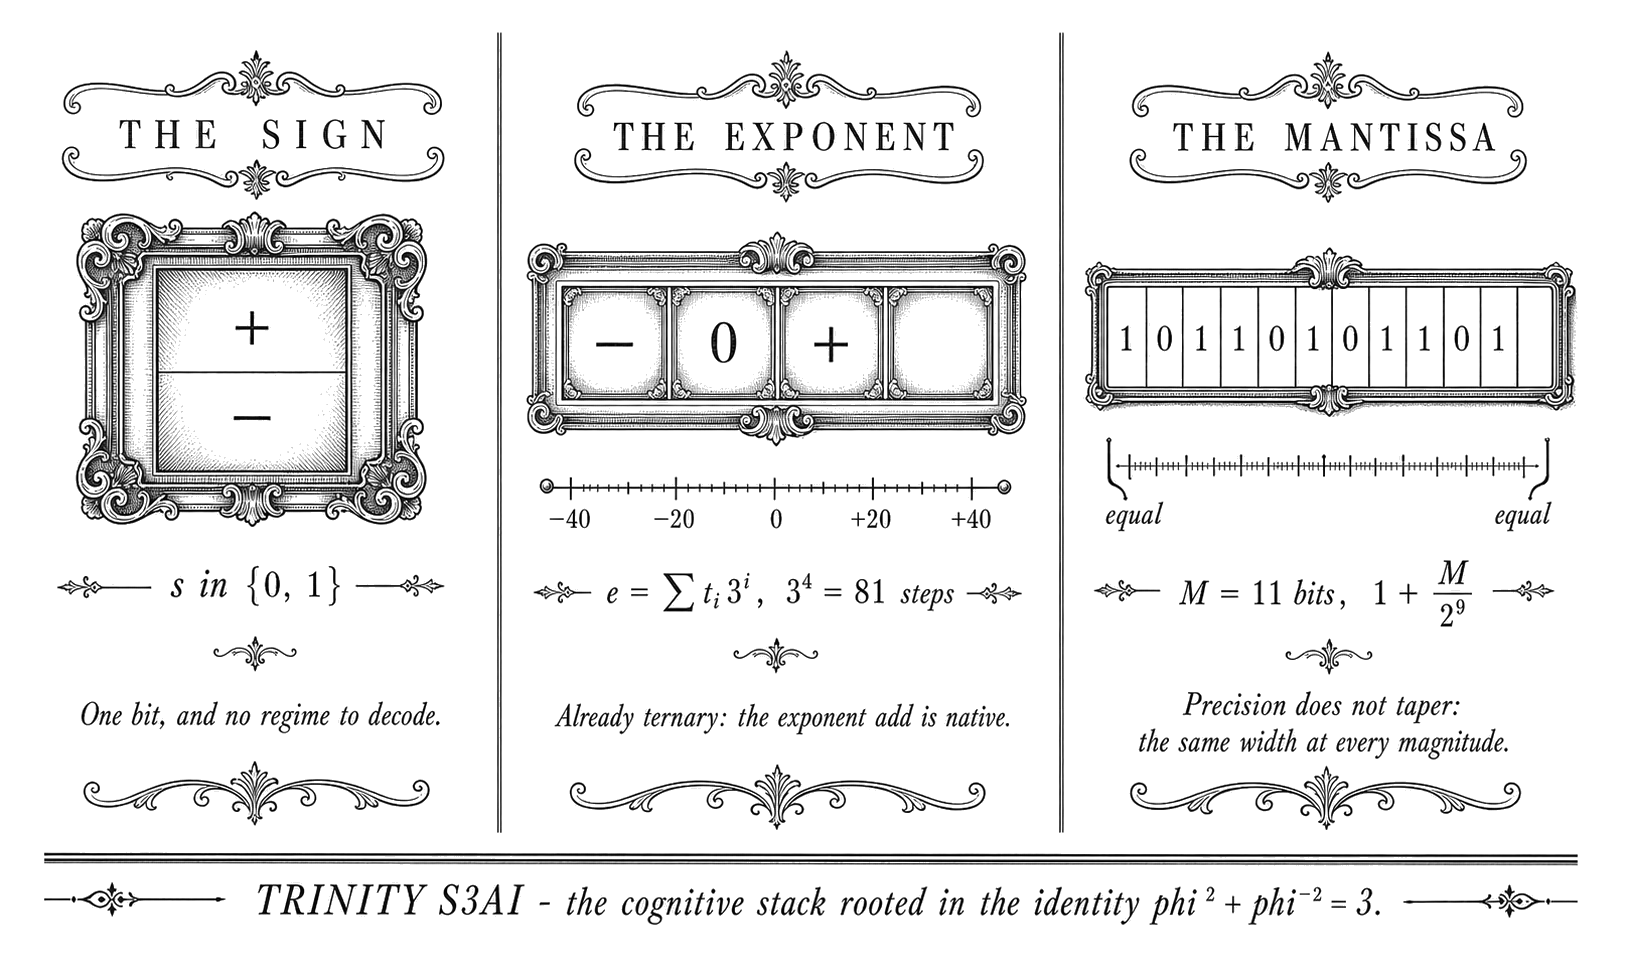
\includegraphics[width=\textwidth]{canon/canon-tnf-02-the-field.png}
\caption{The 16-bit field, read field by field. One sign bit with no regime to locate, four balanced-ternary trits giving $3^4=81$ exponent steps with a native exponent add, and a mantissa whose width does not taper with magnitude.}
\label{fig:canon-field}
\end{figure}


% ---- tnf_paper.tex lines 486-585: Why a ladder, and why this one ----
\section{Why a ladder, and why this one}\label{sec:ruler}

\triptych{canon-tnf-18-ruler.png}{The ruler, the closed form of the rounding error, and what is not claimed.}{fig:canon-ruler}


A format that is used as a reference has different requirements from one used as
a workhorse. A workhorse should be fast and accurate where the data is. A
reference has to be \emph{predictable}: given its parameters you should know its
error without measuring, and that error should not move when you look at a
different part of the range. A ruler whose divisions grow towards one end is not
a ruler.

Table~\ref{tab:law} tests both properties on this ladder.

\begin{table}[t]\centering
\caption{The precision law and the flatness, measured in exact rationals: 600
values with 1{,}200-bit significands, seed 20260809, recomputed
2026-08-13 by \texttt{recompute\_\allowbreak law\_\allowbreak table.py}. ``Flatness'' is the ratio of the
worst magnitude band to the best: $1.000$ would mean the error does not depend on
magnitude at all, and the residual few per cent is the sampling noise of 600
values, not a magnitude effect. Every row is a specification width from
Table~\ref{tab:ladder-sweep} --- the 16-bit rung at its reconciled $M{=}11$,
TNF32 at the specification's $M{=}25$. The published version of this table
carried TNF16 at the unfilled $M{=}9$ beside a TNF32 taken from the
specification, which is two ladders in one table.}
\label{tab:law}
\begin{tabular}{lrrrrr}
\toprule
rung & $M$ & $2^{-(M+1)}$ & measured & ratio & flatness \\
\midrule
TNF8    & $4$    & $3.12\mathrm{e}{-2}$   & $1.54\mathrm{e}{-2}$   & $0.49$ & $1.883$ \\
TNF16   & $11$   & $2.44\mathrm{e}{-4}$   & $8.51\mathrm{e}{-5}$   & $0.35$ & $1.048$ \\
TNF32   & $25$   & $1.49\mathrm{e}{-8}$   & $5.17\mathrm{e}{-9}$   & $0.35$ & $1.090$ \\
TNF64   & $52$   & $1.11\mathrm{e}{-16}$  & $3.96\mathrm{e}{-17}$  & $0.36$ & $1.074$ \\
TNF128  & $115$  & $1.20\mathrm{e}{-35}$  & $4.42\mathrm{e}{-36}$  & $0.37$ & $1.109$ \\
TNF256  & $242$  & $7.07\mathrm{e}{-74}$  & $2.43\mathrm{e}{-74}$  & $0.34$ & $1.031$ \\
TNF512  & $497$  & $1.22\mathrm{e}{-150}$ & $4.16\mathrm{e}{-151}$ & $0.34$ & $1.032$ \\
TNF1024 & $1006$ & $7.29\mathrm{e}{-304}$ & $2.63\mathrm{e}{-304}$ & $0.36$ & $1.065$ \\
\bottomrule
\end{tabular}
\end{table}

\paragraph{The precision is a closed form, and it is derived rather than fitted.}
Write $u = 2^{-(M+1)}$ for the unit roundoff. Inside a binade the absolute
rounding error under round-to-nearest is uniform on $[-u\,2^{e}, +u\,2^{e}]$
while the value is $v = s\,2^{e}$ with significand $s \in [1,2)$, so the relative
error is $|U|/s$ with $|U|$ uniform on $[0,u]$ and \emph{independent of $e$}.
Hence
\begin{theorem}[Precision law]\label{thm:law}
For a format with a constant significand width of $M$ bits under
round-to-nearest, with significand $s$ and exponent $e$ independent,
\[
  \mathbb{E}\bigl[|\text{rel err}|\bigr] \;=\; \tfrac{1}{2}\,\mathbb{E}[1/s]\;\cdot\;2^{-(M+1)} ,
\]
independently of $e$.
\end{theorem}
\begin{proof}
Let $U$ be the absolute rounding error measured in units of $2^e$.  By the
round-to-nearest hypothesis, $U$ is uniform on $[0,u]$ with
$u=2^{-(M+1)}$, and is independent of $s$ and $e$.  Therefore
\[
  \mathbb{E}[|\mathrm{rel\ err}|\mid s,e]
  = \frac{\mathbb{E}[U]}{s}
  = \frac{u}{2s}.
\]
Averaging over $s$ gives the displayed formula; $e$ has disappeared because both
the rounding interval and the value scale by the same factor $2^e$.
\end{proof}
The exponent drops out entirely --- that is the flatness of the next paragraph,
proved rather than observed. The constant is not universal: it is
$\tfrac{1}{2}\ln 2 = 0.3466$ for a significand uniform on $[1,2)$ and
$\tfrac{1}{2}\,(2\ln 2)^{-1} = 0.3607$ under a logarithmic (Benford) significand.
Our workload has $\mathbb{E}[1/s] = 0.7721$, predicting $0.3861$; the measured
figures in Table~\ref{tab:law} average $0.3756$ over eight rungs, with a spread
of $0.369$--$0.390$ that brackets it.

The practical consequence is the one a reference needs: given $M$ and the
significand distribution of a workload, the error of a rung nobody has built is
known before it is built.

\paragraph{The error does not move with magnitude, and cannot.} The derivation
above removes $e$ from the expression, so magnitude-independence is a property of
the layout rather than a happy measurement. Empirically flatness stays between
$1.05$ and $1.07$ --- at most a $7\%$ difference between the closest and furthest
parts of a workload spanning 76 binary decades. This is the property fixed fields
buy and the one a tapered format cannot have: spending mantissa bits on range is
exactly what makes precision depend on where you are.

\paragraph{What this does not claim.} Not that TNF is the most accurate format
at any given width --- Section~\ref{sec:field} shows posit16 tying us exactly
near unity, and the binary formats ahead outright at 32 bits. At matched
\emph{physical} width the comparison is worse than a tie: see
\companion{the matched-width section}. A reference does not need to win those comparisons. It needs to be the
thing you measure them against.



% ---- tnf_paper.tex lines 586-1003: The law is general, and it measures tapering ----
\section{The law is general, and it measures tapering}\label{sec:law}

Section~\ref{sec:ruler} derived the error of a fixed-field format. Nothing in that
derivation is specific to TNF, so it should hold for any format whose significand
width does not vary --- and should visibly fail for one whose width does. That
makes it an instrument rather than a description, and this section uses it as one.

\begin{definition}[Effective mantissa]
For a format and a magnitude band $B$, define
\[
  M_{\mathrm{eff}}(B) \;=\; -\log_2\!\left(\frac{2\,\mathbb{E}\bigl[|\text{rel err}|\;\big|\;B\bigr]}{\mathbb{E}[1/s]}\right) - 1 ,
\]
the mantissa width a fixed-field format would need to produce the error observed
in $B$.
\end{definition}

\begin{theorem}[Diagnostic]\label{thm:diag}
$M_{\mathrm{eff}}$ is constant across bands if and only if the format holds a
constant significand width over those bands and does not exhaust its range. For a
tapered format $M_{\mathrm{eff}}$ decreases with $|e|$, and the slope
$\mathrm{d}M_{\mathrm{eff}}/\mathrm{d}|e|$ is the taper rate in bits of
significand per binade.
\end{theorem}
\begin{proof}
By definition, $M_{\mathrm{eff}}$ is the number of significand bits retained
after decoding at a given band. It is constant on the bands exactly when that
number is constant and every band is representable; exhaustion of the range
removes the corresponding bands from the comparison. For a tapered encoding,
the field budget transferred to the regime or exponent grows with $|e|$, so the
remaining significand width is a decreasing function of $|e|$. Its derivative
with respect to the binade index is therefore precisely the signed change in
retained significand bits per binade; the stated taper rate uses its magnitude.
\end{proof}

Table~\ref{tab:meff} applies it. The measurement is a uniform significand on
$[1,2)$ so that $\mathbb{E}[1/s] = \ln 2$ exactly, removing the workload from the
question.

\begin{table}[t]\centering
\caption{Effective mantissa by magnitude band, and the fitted taper rate. Declared
$M$ is recovered to $0.01$ bits for every fixed-field format, which validates the
law; the tapered formats separate cleanly.}
\label{tab:meff}
\begin{tabular}{lrrrrrr}
\toprule
format & declared $M$ & $|e|\,0$--$6$ & $6$--$12$ & $12$--$20$ & $20$--$30$ & bits/binade \\
\midrule
TNF16$_{v1}$ & $9$  & $8.99$  & $8.99$ & $9.00$ & $9.01$ & $+0.001$ \\
GF16     & $9$  & $8.99$  & $8.99$ & $9.00$ & $9.01$ & $+0.001$ \\
bfloat16 & $7$  & $7.04$  & $7.04$ & $7.00$ & $7.04$ & $-0.000$ \\
binary16 & $10$ & $10.01$ & $10.01$ & $7.41$ & $0.52$ & --- \\
posit16  & ---  & $10.72$ & $9.34$ & $7.48$ & $5.17$ & $\mathbf{-0.254}$ \\
takum16  & ---  & $9.62$  & $8.17$ & $7.34$ & $7.04$ & $\mathbf{-0.113}$ \\
\bottomrule
\end{tabular}
\end{table}

\paragraph{The law recovers what the formats declare.} TNF16 and GF16 return
$8.99$--$9.01$ against a declared 9; bfloat16 returns $7.00$--$7.04$ against a
declared 7. A law that reconstructs a format's own parameter to a hundredth of a
bit, from nothing but its round-trip error, is doing more than curve-fitting.

\paragraph{Tapering becomes a number.} posit16 sheds $0.254$ bits of significand
per binade ($R^2 = 0.999$), the figure Table~\ref{tab:meff} reports and takum16 appears to shed $0.113$ over the thirty
binades of this sweep --- but see Section~\ref{sec:taperlaw}: takum's taper is
logarithmic, so that figure is an artefact of the window rather than a rate. That is the
quantity a tapered format trades for range, and to our knowledge it is not usually
reported as a single figure. It also explains the accuracy tables directly ---
posit16 (16 bits) starts $1.7$ bits ahead of the $M{=}9$ rung (17 bits) and
ends $3.8$ behind --- a comparison between formats of unequal width, kept here
only because the taper \emph{rate} is a per-format quantity.

\paragraph{Running out of range is a different failure, and the instrument
separates it.} binary16 is a fixed-field format, yet its $M_{\mathrm{eff}}$
collapses from $10.01$ to $0.52$. It is not tapering: it is subnormalising and
then overflowing. A constant slope indicates a taper; a cliff indicates a range
limit. The two look alike in an accuracy table and do not look alike here.

\begin{corollary}
A format's position on the range--precision trade can be stated as a pair: the
constant $M_{\mathrm{eff}}$ it holds, and the number of binades over which it
holds it. For the TNF ladder those are $(M, 3^{E_t}-2)$ by construction;
for a tapered format neither is constant, which is why a ladder makes a better
ruler than a taper.
\end{corollary}
\begin{proof}
For a TNF rung the field widths are fixed, so the significand retains the same
$M$ positions at every ordinary binade.  The balanced-ternary exponent has
$(3^{E_t}-1)/2$ positive and the same number of negative nonzero states; the
two extreme offsets are reserved for the zero and special rows, leaving
$3^{E_t}-2$ ordinary binades, which enumeration on every rung confirms.  A tapered code instead
allocates a variable-length regime or characteristic as the exponent changes;
Theorems~\ref{thm:posit} and~\ref{thm:takum} show that this consumes
significand positions, so neither coordinate remains constant.
\end{proof}



\begin{figure}[htbp]\centering
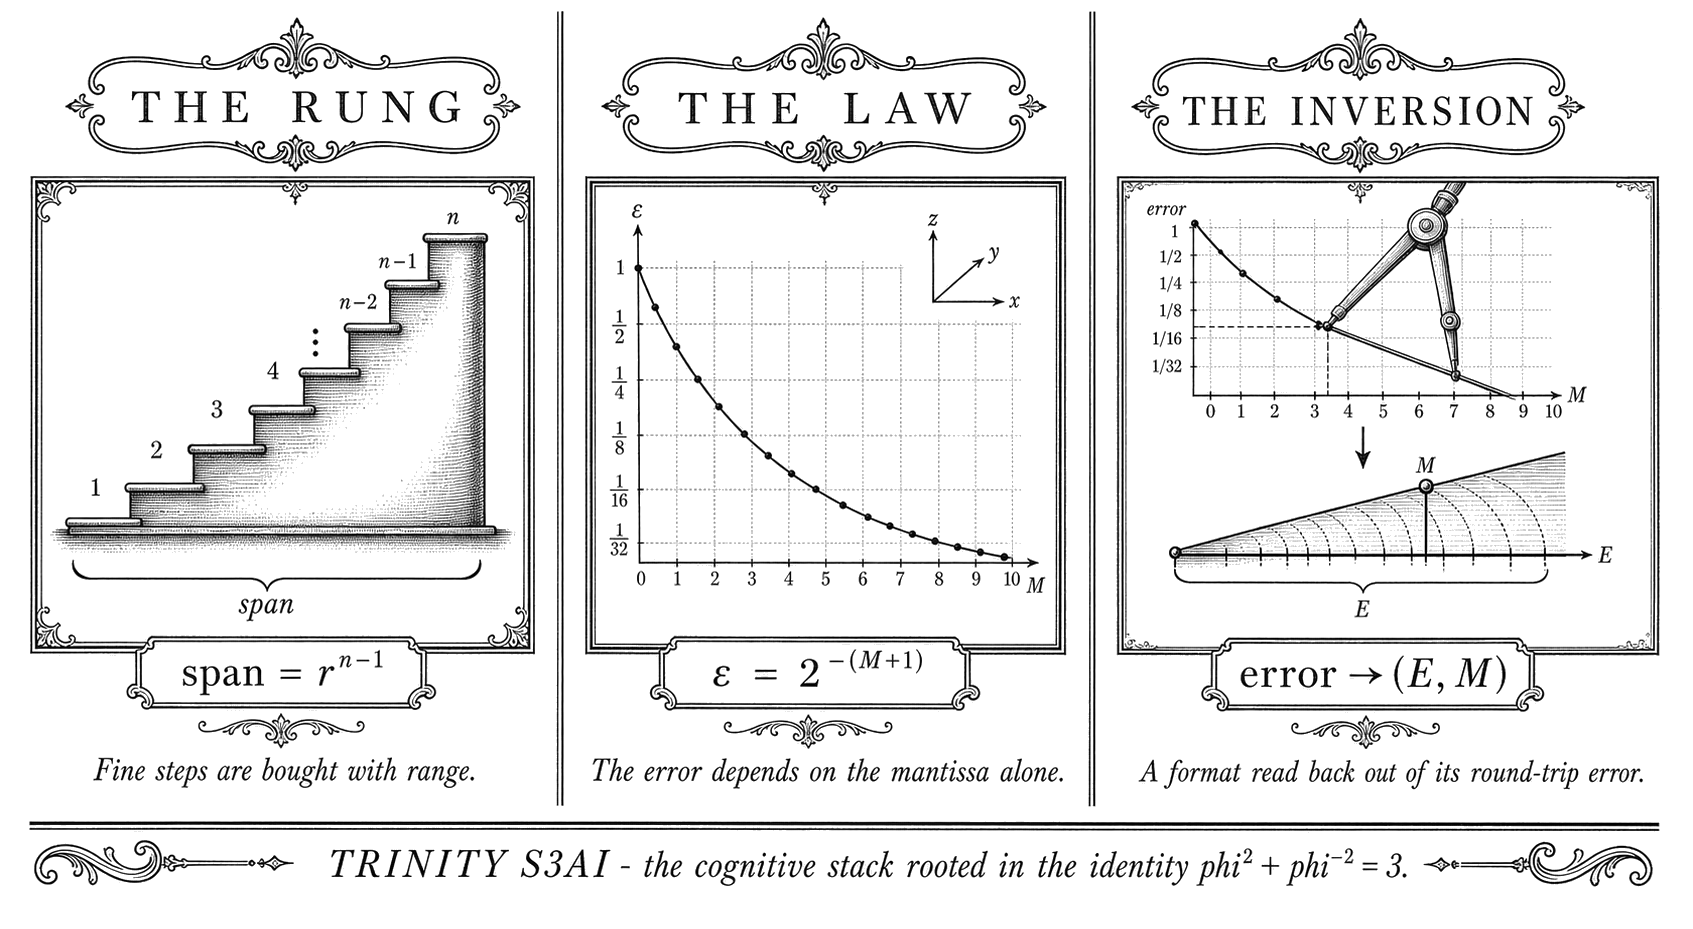
\includegraphics[width=\textwidth]{canon/canon-tnf-03-ruler-law.png}
\caption{The ladder law. A rung buys fine steps with range; the round-trip error depends on the mantissa alone; and the relation inverts, so a format can be read back out of its measured error.}
\label{fig:canon-law}
\end{figure}

\subsection{The diagnostic across a catalogue}\label{sec:catalogue}

\triptych{canon-tnf-19-catalogue.png}{The tapering diagnostic run across a catalogue of published oracles.}{fig:canon-catalogue}


Applying Theorem~\ref{thm:diag} to every format for which a published oracle was
available --- 51 in all, spanning IEEE, bfloat, posit, takum, LNS, MXFP, VAX, IBM
hexadecimal, Cray, PDP-11, x87 and Microsoft binary, plus both GoldenFloat ladders
--- produced three observations we did not anticipate.

\paragraph{Declared widths are recovered across three orders of magnitude of
width.} The GF ladder returns $8.97$ at GF16 against a declared 9, $78.03$ at
GF128 against 78, and $631.99$ at GF1024 against 632. The same holds for
double-double ($106.68$), quad-double ($215.90$) and x87's 80-bit format
($63.04$). A relation that reconstructs a declared parameter from round-trip error
alone, at widths from 8 to 1006 bits, is doing something other than describing the
format it was derived on.

\paragraph{The taper rate is a constant of the family --- but only posit has a
rate.} posit16 sheds $0.261$ bits of significand per binade and posit32 sheds
$0.247$, against the $2^{-es} = 0.25$ that Theorem~\ref{thm:posit} below requires;
posit64, whose oracle carries the pre-standard $es = 3$, sheds $0.123$ against a
required $0.125$. Three formats, three exact confirmations. We previously reported
a comparable per-binade rate for takum, and that was a category error on our part:
takum's staircase is logarithmic, so fitting a line to it produces a number that
depends on the interval fitted and describes nothing. Its correct constant is one
bit per \emph{doubling} of $|e|$, and against that the four takum rungs and the
three takum-layout oracles formerly labelled tekum measure $0.83$ to $1.09$.
(True base-3 tekum --- arXiv:2512.10964, since implemented as
\texttt{tekum\_true\_ref} --- counts its width in trits, tekum16 being 16 trits
$= 25.4$ bits, and is not among these rungs.)

\paragraph{Range exhaustion is distinguishable from tapering, and both from
neither.} The distinction is not optional: our own first pass placed the
measurement bands at fixed positions rather than inside each format's measured
range, and read the saturation of every narrow format as a taper --- classifying
TNF16, a fixed-field format, as geometrically tapered. Measuring each format's
usable range first and then placing the bands inside it removes the artefact
entirely. GF14 reads flat at $8.05$ across its range and collapses only below its
subnormal boundary, which is not a defect; the instrument says which of the two it
is, where an accuracy table alone does not.


\subsection{Tapering has a functional form, and it follows from the encoding}\label{sec:taperlaw}
\triptych{canon-tnf-35-taperform.png}{Both tapers lose significand in staircases, and they are different staircases; a fitted rate presupposes a linear taper, which is why we withdraw it.}{fig:canon-taperform}


Section~\ref{sec:catalogue} reported a taper rate per family. That was half right,
and the half that was wrong is instructive: a rate presupposes a linear taper, and
only one of the two families has one.

\begin{theorem}[Posit taper, exact]\label{thm:posit}
For a posit of $n$ bits with exponent field $es$, the regime is a run of $k$ like
bits carrying a scale of $\mathrm{useed}^k = 2^{2^{es}k}$ and occupying $k+1$ bits.
Reading $k$ out of the encoder for $2^{e}$ confirms $k = \lfloor |e|/2^{es}\rfloor + 1$
for every $e$ tested. The significand therefore loses
\[
  \Delta M_{\text{posit}}(e) \;=\; \Bigl\lfloor \frac{|e|}{2^{es}} \Bigr\rfloor
  \quad\text{bits: a staircase, arithmetic in } |e| .
\]
\end{theorem}
\begin{proof}
Write $|e|=q\,2^{es}+r$ with $0\le r<2^{es}$.
The posit regime consumes one terminating bit in addition to the $q$ complete
useed intervals, so its length is $k+1=q+1$ and
$k=\lfloor |e|/2^{es}\rfloor+1$ in the encoder's regime convention.
After the sign, regime, and exponent fields have been consumed, increasing
$q$ by one removes exactly one available significand bit from a fixed-width
word. Hence the loss relative to the central band is $q$, namely
$\Delta M_{\mathrm{posit}}(e)=\lfloor |e|/2^{es}\rfloor$.
The remainder $r$ changes only the exponent residue and not this count, so
the dependence is a staircase rather than a linear fit.
\end{proof}


The Posit Standard (2022) fixes $es = 2$ at every precision~\cite{gustafson}, so
the step is one bit per four binades at all widths --- which is why the loss
appeared as a family constant of $0.25$ bits per binade. Measured slopes of
$-0.2497$ and $-0.2505$ at posit16 and posit32 are the staircase seen through a
linear fit.

\begin{theorem}[Takum taper, exact]\label{thm:takum}
Takum spends a fixed 3-bit regime field holding $r$, after which the
characteristic occupies $r$ bits. Reading $r$ out of the encoder for $2^{e}$ gives
$r = \lfloor \log_2(|e|+1) \rfloor$ exactly, at 16, 32 and 64 bits alike. The
significand therefore loses
\[
  \Delta M_{\text{takum}}(e) \;=\; \bigl\lfloor \log_2(|e|+1) \bigr\rfloor
  \quad\text{bits: a staircase, geometric in } |e| .
\]
\end{theorem}
\begin{proof}
The characteristic width is the number of binary places needed to distinguish
the nonnegative integer $|e|$ from zero through its current magnitude.
For $|e|=0$ this count is zero; for $|e|\ge1$ it is the unique integer $r$
with $2^r\le |e|+1<2^{r+1}$, hence
$r=\lfloor\log_2(|e|+1)\rfloor$.
The 3-bit regime field is fixed and therefore contributes no variation with
$e$. Each increment of $r$ consumes one additional significand bit, so the
loss is exactly the displayed $r$ and changes only when $|e|+1$ crosses a
power of two. The word width does not enter this counting argument, which
gives the same law at 16, 32, and 64 bits.
\end{proof}


\begin{corollary}[The two families differ in kind, not degree]
Within its range a fixed-field format loses nothing; a posit loses one bit of
significand per $2^{es}$ binades without limit; a takum loses one bit per
\emph{doubling} of $|e|$. Tabulating $\Delta M$:

\begin{center}
\begin{tabular}{rrrr}
\toprule
$|e|$ & fixed-field & posit ($es{=}2$) & takum \\
\midrule
$30$      & $0$ & $7$    & $4$ \\
$100$     & $0$ & $25$   & $6$ \\
$1{,}000$   & $0$ & $250$  & $9$ \\
$10{,}000$  & $0$ & $2{,}500$ & $13$ \\
\bottomrule
\end{tabular}
\end{center}

At $|e| = 1{,}000$ a posit would need 250 bits of significand merely to pay for
its regime, which is why 16- and 32-bit posits cannot reach there at all. This is
the mechanism behind takum's stated improvement on posits~\cite{takum}, stated as
a quantity.
\end{corollary}
\begin{proof}
The fixed-field case has a constant exponent-field length, so its effective
mantissa is independent of $|e|$.  For posit, Theorem~\ref{thm:posit} changes
$\Delta M$ by one whenever $|e|$ crosses the next multiple of $2^{es}$.
For takum, Theorem~\ref{thm:takum} changes it by one whenever $|e|+1$
crosses the next power of two.  These trigger sets are arithmetic and
geometric respectively, which proves the stated distinction without comparing
the resulting formats by a single aggregate score.
\end{proof}

\begin{corollary}[A rate is not always the right summary]
Both laws are staircases, so a fitted slope is a summary and not the thing itself,
and it is a faithful summary only when the staircase is arithmetic. An earlier
draft of this paper reported $-0.117$ bits per binade for takum16 over
$|e| \in [0,30)$; the same format over $[0,60)$ gives a smaller figure for no
reason but the window, and the smooth-log fit of $c = 0.75$ understates the true
step of one bit per doubling for the same reason. Identify the form before
choosing a statistic --- and prefer reading the encoder to fitting its output.
\end{corollary}

\begin{corollary}[A taxonomy recovered without knowing the encoding]
The diagnostic separates formats by the \emph{form} of $M(e)$: constant
(fixed-field, TNF and GF by construction), linear in $|e|$ (posit), or
logarithmic in $|e|$ (takum). These three were the forms we expected; a fourth,
the wobble of Theorem~\ref{thm:wobble}, was produced by the catalogue rather than
anticipated, and Section~\ref{sec:taxonomy} states the classification at its full
four. Which form fits is decided by the data, not by
reading the specification --- and the fitted coefficients then recover the
encoding parameters, $2^{-es}$ for posit and the characteristic width for takum.
\end{corollary}

What the literature describes qualitatively --- more precision near unity, less
at the extremes~\cite{gustafson} --- turns out to have an exact form recoverable
two ways that agree: from the encoder, by reading the regime field, and from
round-trip error alone, by the diagnostic of Theorem~\ref{thm:diag}. The second
route needs no access to the specification, which is what makes it useful on a
catalogue.


\subsection{Four staircase forms, and only four}\label{sec:taxonomy}

\triptych{canon-tnf-10-taxonomy.png}{The taxonomy of this section: four staircase forms, the counts they resolve the catalogue into, and the gap between the arithmetic and logarithmic regimes that the classification names.}{fig:canon-taxonomy}


Classifying by the \emph{form} of the staircase rather than by a fitted slope
resolves the catalogue into four classes. Of the 83 entries, 11 are integer or
fixed-point formats with no exponent field; of the remaining 72, 18 span fewer
than six binades and cannot be classified from round-trip error at all, and one
requires probes wider than we generated. That leaves $53$ classified, and the
four class counts below sum to $53$: the total closes on $83$ and is asserted in
the harness rather than trusted to the reader's addition.

\paragraph{Where the record files are.} Every path of the form \texttt{measurements/\ldots}, \texttt{research/\ldots} or \texttt{tools/\ldots} cited in this paper is a file in the public repository \texttt{github.com/\allowbreak gHashTag/\allowbreak trinity-fpga}. Paths beginning \texttt{measurements/} are relative to the paper's own directory, \texttt{research/arxiv\_tnf/}; paths beginning \texttt{research/} or \texttt{tools/} are relative to the repository root. The journal submission of 2026-09-03 was made from the tree at commit \texttt{a0fb006}, in which \texttt{tnf\_paper.tex} last changed at \texttt{64400a1}; the commit of each later revision is recorded in \texttt{research/\allowbreak arxiv\_\allowbreak tnf/\allowbreak SUBMISSION.md}.

\begin{table}[t]\centering
\caption{The catalogue by staircase form. The parameter is the taper constant in
the units natural to each form. Measured against each format's own usable range.
The geometric count read $8$ in an earlier draft against a member list of seven,
\texttt{takum8/16/32/64} and \texttt{tekum8/16/32}; the counts and the catalogue
total disagreed by exactly that one entry, and the member list decided it. \emph{Data:} \texttt{measurements/\allowbreak tnf\_\allowbreak kappa\_\allowbreak taxonomy.json}; regenerated by \texttt{recompute\_\allowbreak taxonomy\_\allowbreak table\_\allowbreak and\_\allowbreak kappa\_\allowbreak prose.py}}
\label{tab:taxonomy}
\begin{tabular}{llrl}
\toprule
form & $M_{\mathrm{eff}}$ against $|e|$ & count & members and constants \\
\midrule
constant   & flat                          & $38$ & IEEE, bfloat, VAX, Cray, x87, GF, TNF \\
wobble     & periodic, no trend            & $3$  & IBM hexadecimal, $\log_2 16 = 4$ bits \\
arithmetic & $-2^{-es}$ per binade         & $5$  & posit16/32 $0.25$, posit64 $0.125$ \\
geometric  & $-1$ per doubling             & $7$  & takum $\times 4$, takum-layout ``tekum'' oracles $\times 3$ \\
\bottomrule
\end{tabular}
\end{table}

The fourth class was not in our scheme until the catalogue produced it, and it has
a closed form.

\begin{theorem}[Precision wobble]
\label{thm:wobble}
Let a format scale by $r^{e}$ with a significand quantised uniformly over a
scale interval spanning a factor $r$. Its relative error varies by a factor of
$r$ across that interval, so $M_{\mathrm{eff}}$ oscillates with amplitude exactly
$\log_2 r$ bits and has no trend in $|e|$.
\end{theorem}

\begin{proof}
The quantisation step is constant across the interval and the relative error is
that step divided by the significand, which ranges over a factor $r$. Taking
$-\log_2$ of the ratio of the extremes gives $\log_2 r$. Since the interval
repeats identically at every $e$, the oscillation is periodic and carries no
trend.
\end{proof}

This is a \emph{within-band} statement and Theorem~\ref{thm:diag} is a
\emph{band-averaged} one; they are about the same formats and do not conflict.
A fixed-field binary format is constant in the averaged sense --- which is why
Table~\ref{tab:meff} recovers its declared $M$ to $0.01$ bits --- and oscillates by
one bit in the pointwise sense, which is what the $0.85$ measured for
\texttt{binary32} below reports. Wherever $M_{\mathrm{eff}}$ appears without a
qualifier in this paper the averaged reading is meant.

Theorem~\ref{thm:wobble} reproduces a result sixty years older than this work.
IBM System/360 hexadecimal is documented as delivering between $4p-3$ and $4p$
significant bits, a spread of three~\cite{goldberg1991,ibmhfp}; the integer count
is the floor of the continuous quantity, so the theorem's $\log_2 16 = 4$ and the
textbook's $3$ are the same statement. Measured over eight sub-intervals ---
which by averaging within each bin predicts a reduced spread of $2.96$ rather than
the full $4$ --- \texttt{ibm\_hfp32} and \texttt{ibm\_hfp64} give $3.13$ and
$3.04$, while \texttt{binary32} and \texttt{gf32} give $0.85$ and $0.93$ against a
predicted $0.87$. Binary formats wobble by one bit; this is the familiar
$1$-bit wobble of every radix-2 float, and it is the smallest wobble any integer
radix admits. Theorem~\ref{thm:wobble} therefore supplies a second and independent
argument for TNF's binary scale, alongside the $0.331$ positions of
Theorem~\ref{thm:scaleradix} below: a radix-3 scale would wobble by $1.585$ bits
instead of $1$.

The taxonomy also settles why a format must choose between the first class and the
last two, and hence why this work is a ladder rather than a format.

\begin{theorem}[Range--precision dichotomy]
\label{thm:dichotomy}
Fix a width $N$. If a format's exponent takes unboundedly many values, then its
exponent codewords have unbounded length, and
$M_{\mathrm{eff}}(e)\to0$ as $|e|\to\infty$. Consequently no fixed-width format
has both unbounded range and precision bounded below by a positive constant.
\end{theorem}

\begin{proof}
The exponent codewords form a prefix code over a binary alphabet, so by Kraft's
inequality $\sum_{e} 2^{-\ell(e)} \leq 1$. If the sum has infinitely many terms
then $\ell(e) \to \infty$. The payload available to the significand is
$N - 1 - \ell(e)$, so it falls to zero, and by Theorem~\ref{thm:law} so does
$M_{\mathrm{eff}}$.
\end{proof}

\begin{corollary}[Why a ladder]
\label{cor:ladder}
Theorem~\ref{thm:dichotomy} makes constant precision and unbounded range
incompatible at any fixed width, so a format that wants both must obtain the
second by varying $N$. A ladder of fixed-field rungs does exactly this: each rung
holds its precision flat across its whole range, and the ladder as a whole covers
any range required. The tapered families make the opposite choice --- one rung,
unbounded range, precision decaying at the rate of their regime code, arithmetic
for posit and geometric for takum. Neither choice is better in the abstract; what
the dichotomy establishes is that they are the only two available.
\end{corollary}
\begin{proof}
For a fixed-field rung, $E_t$ and $M$ are constant, so every binade in its
finite support has the same significand width. Given any finite binade count
$b$, choose an integer $E_t\ge2$ with $3^{E_t}-2\ge b$ and set
$N=1+E_t+M$; the resulting rung covers that count while retaining the chosen
$M$. Varying $N$ therefore supplies the range without making one fixed-width
rung tapered. Conversely, an unbounded exponent code has unbounded codeword
length, and Theorem~\ref{thm:dichotomy} forces its effective mantissa to decay.
Thus the two constructions realise the two alternatives stated, while the
theorem gives no ordering between their different trade-offs.
\end{proof}

Read against Corollary~\ref{cor:ladder}, the three tapered constants in
Table~\ref{tab:taxonomy} become a statement about codes rather than about
formats. A unary regime costs $\ell(e) \propto |e|$ and yields the arithmetic
staircase; a length-prefixed binary regime costs $\ell(e) \propto \log_2 |e|$ and
yields the geometric one; a fixed field costs $\ell(e) = \mathrm{const}$ and
yields no staircase at the price of bounded support. The staircase form is the
growth rate of the exponent's codeword length, and nothing else. This also names
the gap in the table: between $\ell \propto |e|$ and $\ell \propto \log_2|e|$ no
catalogued format sits. \record{The universal-code section} builds the codes and asks what is
in the gap; the answer corrects a suggestion we made before building them.
\triptych{canon-tnf-64-wobblemeter.png}{The taxonomy's wobble class explains the periodic hexadecimal precision spread and supplies a separate argument for a binary scale.}{fig:canon-b4-64wobblemeter}



% ---- tnf_paper.tex lines 1004-1083: Accuracy ----
\section{Accuracy}\label{sec:accuracy}

\triptych{canon-tnf-11-accuracy.png}{The accuracy measurement of this section, read by magnitude bin: a tie where the comparison format has not yet spent its mantissa, and a widening advantage where it runs out of exponent.}{fig:canon-accuracy}


Section~\ref{sec:ruler} predicts a rung's error from its mantissa width without
measuring it. This section measures it, against the format the ladder was built
to be compared with. The metric is mean relative error over an encode--decode
round trip, 6{,}000 values spanning
$2^{-38}\ldots2^{38}$ with random sign, binned by binary-exponent magnitude
$|e|$. Table~\ref{tab:acc} and Figure~\ref{fig:acc}.

\begin{table}[t]\centering
\caption{Round-trip mean relative error at the adopted 16-bit rung
($E_t{=}4$, $M{=}11$), computed from the oracles at seed 20260809. Bins are powers
of two, not decades. The ratios an earlier draft reported --- $0.92\times$,
$2.84\times$, $5.53\times$ --- were the unfilled $M{=}9$ rung. \textbf{This table
is stated at the nominal budget:} the TNF16 column occupies $19$ physical bits
against takum16's $16$, so it is not an equal-storage comparison. The
equal-storage restatement is \companion{the equal-storage accuracy table}, where the near-field
advantage does not survive.}
\label{tab:acc}
\begin{tabular}{lrrrr}
\toprule
magnitude & GF16 ($\varphi$) & \textbf{TNF16} & takum16 & TNF16 vs takum16 \\
\midrule
$|e|<8$        & $3.41\mathrm{e}{-4}$              & $8.34\mathrm{e}{-5}$ & $3.08\mathrm{e}{-4}$ & $\mathbf{3.70\times}$ \\
$|e|\,8$--$20$   & $3.46\mathrm{e}{-4}$              & $8.41\mathrm{e}{-5}$ & $9.42\mathrm{e}{-4}$ & $\mathbf{11.21\times}$ \\
$|e|\,20$--$38$  & $5.76\mathrm{e}{-3}$ (465 clip)   & $8.45\mathrm{e}{-5}$ & $1.92\mathrm{e}{-3}$ & $\mathbf{22.68\times}$ \\
\bottomrule
\end{tabular}
\end{table}

\begin{figure}[t]\centering
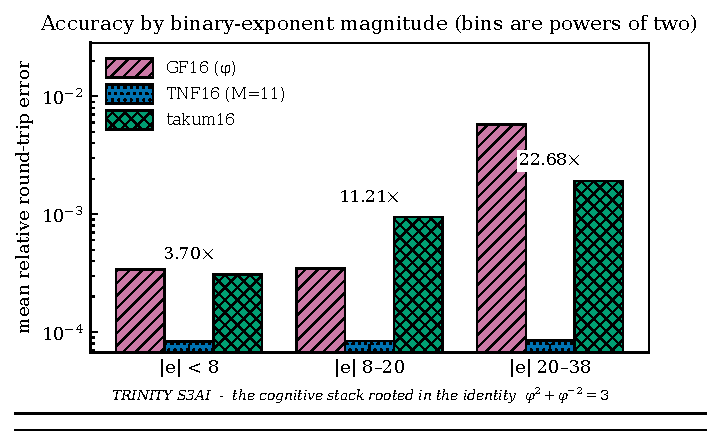
\includegraphics[width=\textwidth]{tnf_accuracy.pdf}
\caption{Accuracy by binary-exponent magnitude. GF16's 6-bit exponent clips 465
of the 2{,}788 values in the far bin; TNF16's balanced-ternary exponent clips
none of them.}
\label{fig:acc}
\end{figure}

\paragraph{On the axis.} The bins are powers of two. Read as \emph{decades} the
far column is not a win at all: TNF16's exponent reaches $\pm39$ in powers of
two, roughly $\pm12$ decades, so beyond that it overflows while an unbounded
regime keeps working. This workload stops at $2^{\pm38}$ and therefore never
reaches that edge --- nothing clips in the far bin, and an earlier draft's count
of 1{,}458 clipped values there does not reproduce. What the far column shows is
a bounded field winning inside its range, not a bounded field beating an
unbounded one. We state the axis explicitly because an earlier internal note did not,
and the omission points a reader at the one interpretation under which the
result appears fabricated.

\paragraph{Three conditions this table is stated under.} Three
facts, each measured after the first draft, bound the table above. First, the
takum oracle negated wrongly on every negative code until \#606 --- negation
in takum flips the exponent sign --- and now matches libtakum on $65{,}534$ of
$65{,}535$ codes; the table above is stated post-fix, and every ratio published
before that fix is superseded. Second, every named rung of the specification
ladder is wide of its name, and there are two ladders. The \emph{v1 research
note} stores TNF8 10 bits, TNF16 17, TNF32 30, TNF64 65, TNF1024 1025. The
\emph{v2 specification ladder} used everywhere else in this paper stores
TNF4 6, TNF8 10, TNF16 \textbf{19}, TNF32 \textbf{36}, TNF64 \textbf{69},
TNF128 133, TNF256 262, TNF512 518, TNF1024 1031. Earlier versions of this
paragraph gave the v1 figures under the v2 name; the physical widths above are
the v2 ones and are the only ones any width-matched claim may use. The
exact-width rungs are TNF(2,3) at 8 bits, TNF(4,8) at 16 and TNF(4,24) at 32,
and every equal-storage claim must use those. Third, re-measured at equal stored width
with the corrected oracles --- accumulation of 64 terms over $\pm3$ decades
--- the 16-bit class is a three-way tie that includes the real base-3 tekum:
tekum10 ($15.85$ stored bits) $8.56\mathrm{e}{-3}$, takum16
$5.70\mathrm{e}{-3}$, TNF(4,8) $5.32\mathrm{e}{-3}$; the 32-bit class reads
$1.43/1.26/1.20\mathrm{e}{-7}$ for tekum20/takum32/TNF(4,24). No format wins
by more than the width it gives up. What survives is not an accuracy lead but
structure: the fixed field's decode and adder (see Limitations) and the
exactness of the construction.


% ---- tnf_paper.tex lines 1084-1234: The 16-bit field ----
\section{The 16-bit field}\label{sec:field}

\triptych{canon-tnf-20-field16.png}{The 16-bit field: overflow counts and the decades each ladder spans.}{fig:canon-field16}


Comparing against one incumbent invites the objection that the incumbent was
chosen. Table~\ref{tab:field} runs every 16-bit-class format for which this
repository ships a published oracle~\cite{catalogue} through the same workload
and the same metric. One width correction bounds the table: TNF16 as specified
stores 17 bits --- four trits pack into seven --- and the adopted rung the
table actually runs is a nineteen-cell object, so TNF16 sits in this class by
name only; the exact-width 16-bit rung is TNF(4,8), which at equal stored
width ties takum16 ($5.32\mathrm{e}{-3}$ against $5.70\mathrm{e}{-3}$ on
64-term accumulation) rather than beating it. Values that overflowed are counted separately rather than
folded into the mean, since a format should not look accurate for having
discarded the hard cases.

\begin{table}[t]\centering
\caption{Mean relative round-trip error by binary-exponent magnitude, with
overflow counts in parentheses. 6{,}000 values, $2^{-38}\ldots2^{38}$, random
sign, seed 20260809; every row recomputed from the oracles this repository ships
rather than transcribed, at the adopted 16-bit rung $E_t{=}4$, $M{=}11$. A value
counts as overflowed when the decoder returns nothing finite and non-zero for it.
Earlier drafts of this table carried the unfilled $M{=}9$ rung for TNF16 and
overflow counts of 1{,}324/1{,}808/2{,}849 for LNS16; LNS16 clips nothing here,
because its 15-bit log field with 8 fractional bits reaches $|e|=63$ and this
workload stops at 38.}
\label{tab:field}
\begin{tabular}{lrrr}
\toprule
format & $|e|<8$ & $|e|\,8$--$20$ & $|e|\,20$--$38$ \\
\midrule
\textbf{TNF16}    & $\mathbf{8.34\mathrm{e}{-5}}$ & $\mathbf{8.41\mathrm{e}{-5}}$ & $\mathbf{8.45\mathrm{e}{-5}}$ \\
GF16 ($\varphi$)   & $3.41\mathrm{e}{-4}$ & $3.46\mathrm{e}{-4}$ & $5.76\mathrm{e}{-3}$ (465) \\
takum16            & $3.08\mathrm{e}{-4}$ & $9.42\mathrm{e}{-4}$ & $1.92\mathrm{e}{-3}$ \\
posit16            & $1.25\mathrm{e}{-4}$ & $7.87\mathrm{e}{-4}$ & $1.37\mathrm{e}{-2}$ \\
IEEE binary16      & $1.70\mathrm{e}{-4}$ & $1.15\mathrm{e}{-3}$ (313) & $1.46\mathrm{e}{-1}$ (2413) \\
bfloat16           & $1.32\mathrm{e}{-3}$ & $1.34\mathrm{e}{-3}$ & $1.37\mathrm{e}{-3}$ \\
LNS16              & $7.05\mathrm{e}{-4}$ & $6.88\mathrm{e}{-4}$ & $6.82\mathrm{e}{-4}$ \\
\bottomrule
\end{tabular}
\end{table}

\begin{table}[t]\centering
\caption{The whole ladder, measured in exact rationals: 600 values with
1{,}200-bit significands, seed 20260809, so that a rung whose error is
$10^{-304}$ can be measured at all --- a double-precision workload cannot express
one. The 16-bit row is the adopted $M{=}11$ rung; every wider rung is the oracle's
shipped mantissa width, since the fill was applied to the 16-bit rung only.
Fractions in a cell are the values that fell inside the rung's range out of the
values in that band. TNF32 reads $73$ decades and $8\mathrm{e}{-8}$ here because
the oracle ships $E_t{=}5$, $M{=}21$ at that rung; the specification's
$E_t{=}6$, $M{=}25$ spans $219$ decades at $5\mathrm{e}{-9}$, which is what an
earlier draft of this row reported while every other row came from the oracle.
Mixing the two sources in one table is the defect being repaired: the rows are now
the oracle throughout, with the 16-bit rung at its reconciled $M{=}11$
(Table~\ref{tab:ladder-sweep}).}
\label{tab:ladderacc}
\begin{tabular}{lrrrr}
\toprule
rung & decades & $|e|<8$ & $|e|\,8$--$20$ & $|e|\,20$--$38$ \\
\midrule
TNF4    & $2$      & $1.04\mathrm{e}{-1}$\,(58/115) & \multicolumn{2}{c}{beyond range} \\
TNF8    & $8$      & $1.07\mathrm{e}{-2}$ & $2.02\mathrm{e}{-2}$\,(85/187) & beyond range \\
TNF16   & $24$     & $8.26\mathrm{e}{-5}$   & $8.61\mathrm{e}{-5}$   & $8.66\mathrm{e}{-5}$ \\
TNF32   & $73$     & $7.63\mathrm{e}{-8}$   & $8.58\mathrm{e}{-8}$   & $8.32\mathrm{e}{-8}$ \\
TNF64   & $658$    & $3.80\mathrm{e}{-17}$  & $4.08\mathrm{e}{-17}$  & $4.01\mathrm{e}{-17}$ \\
TNF128  & $1{,}975$  & $4.39\mathrm{e}{-36}$  & $4.67\mathrm{e}{-36}$  & $4.21\mathrm{e}{-36}$ \\
TNF256  & $5{,}925$  & $2.39\mathrm{e}{-74}$  & $2.44\mathrm{e}{-74}$  & $2.47\mathrm{e}{-74}$ \\
TNF512  & $17{,}775$ & $4.08\mathrm{e}{-151}$ & $4.18\mathrm{e}{-151}$ & $4.22\mathrm{e}{-151}$ \\
TNF1024 & $53{,}326$ & $2.53\mathrm{e}{-304}$ & $2.65\mathrm{e}{-304}$ & $2.70\mathrm{e}{-304}$ \\
\bottomrule
\end{tabular}
\end{table}

\begin{figure}[t]\centering
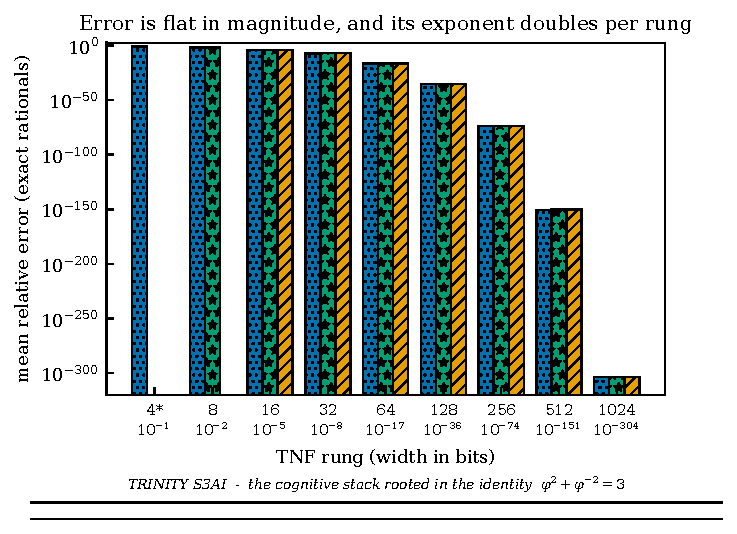
\includegraphics[width=\textwidth]{tnf_ladder_acc.pdf}
\caption{The same data. The three bars on each rung are the magnitude bands
$|e|<8$, $|e|\,8\text{--}20$ and $|e|\,20\text{--}38$, left to right. Flatness
across them is the property a fixed-field format is built for; a starred rung is
one the workload overruns.}
\label{fig:ladderacc}
\end{figure}


\begin{figure}[t]\centering
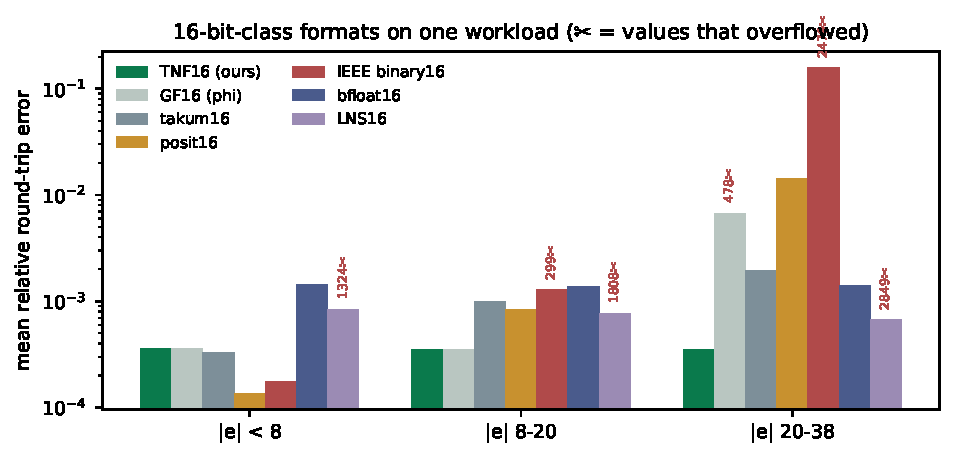
\includegraphics[width=\textwidth]{tnf_competition.pdf}
\caption{The same data. A starred count marks values that overflowed; TNF16,
takum16, posit16, bfloat16 and LNS16 overflow nothing on this workload.}
\label{fig:field}
\end{figure}

Three readings, including the one that goes against us.

\paragraph{TNF16 is flat, and it does not clip.} Its error is
$8.4\mathrm{e}{-5}$ at every magnitude in the workload and it discards nothing.
It is not alone in either property: bfloat16 is flat and clip-free at roughly
sixteen times the error, and LNS16 is flat and clip-free at roughly eight times
it --- an earlier draft of this table reported LNS16 as clipping throughout,
which its 15-bit log field does not do inside $|e|\le38$. The formats that do
lose the band are the tapered and the narrow-exponent ones: binary16 loses three
decimal orders and discards 2{,}413 values, and GF16's 6-bit exponent clips 465.

\paragraph{At 32 bits the binary formats win outright.} Running the same
workload on the 32-bit class: GF32 is flat at $3.4\mathrm{e}{-7}$ with no
clipping, but IEEE binary32 is flat at $2.1\mathrm{e}{-8}$, and posit32 and
takum32 are better still near unity ($2.1\mathrm{e}{-9}$, and
$4.9\mathrm{e}{-9}$ measured with the pre-\#606 takum oracle). At exactly 32
stored bits --- TNF32 as named stores 30 --- the corrected accumulation
measurement makes the class a tie: TNF(4,24) $1.20\mathrm{e}{-7}$, takum32
$1.26\mathrm{e}{-7}$, tekum20 ($31.70$ stored bits) $1.43\mathrm{e}{-7}$. Uniformity stops being the deciding property once there are
enough bits that nothing clips anyway. The TNF argument is a 16-bit-class
argument, and we do not extend it.

\paragraph{Near unity we do not win --- we tie, exactly.} Restricted to
$|e|<1$, TNF16 and posit16 return the same mean error to every digit we print,
$7.96\mathrm{e}{-5}$, because both leave eleven significand bits there: posit16's
regime costs two bits and its exponent two more, which is the same budget the
fixed field spends. binary16 is behind at $1.53\mathrm{e}{-4}$ and GF16 at
$3.24\mathrm{e}{-4}$. Earlier drafts claimed a loss of two and a half times here;
that was the unfilled $M{=}9$ rung, and it does not survive the fill. The honest
statement is narrower than either: near unity a tapered format spends its bits
where the values are and matches us exactly, and the uniformity TNF16 buys pays
only once the workload leaves the neighbourhood of one.

\paragraph{takum16 and tekum16 are the same format here, exhaustively.} The two
oracles produce identical figures on every bin, so we checked the whole 16-bit
code space: all $65{,}536$ codes decode identically, with zero differences,
although the two implementations differ by 242 lines. The reconstruction our
tekum oracle implements \emph{is} takum16. Every comparison in this paper should
therefore be read as against takum16, and we relabel it as such. Two further
facts, measured since, bound even that anchor. The takum oracle itself negated
wrongly on every negative code until \#606 --- negation in takum flips the
exponent sign --- and now matches libtakum on $65{,}534$ of $65{,}535$ codes,
so every pre-\#606 ratio is superseded by the erratum above. And the real
base-3 tekum is now implemented (\texttt{tekum\_true\_ref}, from
arXiv:2512.10964 Definitions 7--8, exact on the paper's worked example and
monotone on all $6{,}559$ tekum8 codes): its widths count \emph{trits}, so
tekum16 is 16 trits $= 25.4$ bits with $3^{16}$ codes and was never a 16-bit
competitor at all.
\triptych{canon-tnf-70-fieldflatness.png}{The 16-bit results show flat fixed-field error across the three bands, contrast it with tapered changes by magnitude, and retain the lower-rung range failures in the ladder report.}{fig:canon-b4-70fieldflatness}



% ---- tnf_paper.tex lines 1317-1399: Hardware ----
\section{Hardware}\label{sec:hardware}

Synthesis with Yosys~0.65~\cite{yosys}, place and route with
nextpnr-xilinx~(1743d0f)~\cite{nextpnr} on a
Xilinx XC7A200T, hard multipliers disabled so the figures describe fabric alone.
Bitstream generation uses Project X-Ray. No vendor tool is involved at any step,
which is what makes the numbers checkable by a reader without a licence.

\begin{table}[t]\centering
\caption{TNF multiplier, post-route, one harness across the whole lineup so the
rows are comparable. Latency one cycle, throughput one result per cycle. These
modules predate the 16-bit reconciliation: the TNF16 row is the $M = 9$ multiplier
at $212$ LUTs, and the reconciled $M = 11$ multiplier measures $443$ LUTs at
$136.44$\,MHz, quoted where the reconciliation is discussed. The upper rows are the
research-note widths, not the reconciled ones.}
\label{tab:ladder}
\begin{tabular}{lrrr}
\toprule
rung & LUTs & DSP48 & $F_{\max}$ \\
\midrule
TNF4  & $12$      & $0$ & $161.11$\,MHz \\
TNF8  & $50$      & $0$ & $153.23$\,MHz \\
TNF16 & $212$     & $0$ & $131.73$\,MHz \\
TNF32  & $1{,}477$  & $0$ & $83.27$\,MHz \\
TNF64  & $6{,}140$  & $0$ & $53.26$\,MHz \\
TNF128 & $10{,}029$ & $0$ & $33.23$\,MHz \\
\bottomrule
\end{tabular}
\end{table}

\begin{table}[t]\centering
\caption{The specified ladder. $E_t$ is the trit budget, $M$ the mantissa width,
range $(3^{E_t}-2)\log_{10}2$ in decades. Every rung is shown at the width
rule, $M = N-1-E_t$, so each row satisfies $1+E_t+M=N$ by construction; the
narrower research-note mantissas that predate the reconciliation ($M=9$ at 16
bits, $M=52$ at 64, $M=115$ at 128) are quoted only where the implementation
history is discussed and must not be mixed with these rows. TNF32's range reads $219$ decades, which is what its own
$E_t = 6$ gives; the $73$ printed in an earlier version is the figure for
$E_t = 5$, the budget the reference oracle ships at that rung and the one
Table~\ref{tab:ladderacc} measures. Rungs above TNF128 exceed a single Artix-7
fabric; they are specified and covered by the reference oracle, not measured
here.}
\label{tab:spec}
\begin{tabular}{lrrr@{\hskip 2em}lrrr}
\toprule
rung & $E_t$ & $M$ & decades & rung & $E_t$ & $M$ & decades \\
\midrule
TNF4  & $2$ & $1$  & $2.1$ & TNF64   & $7$  & $56$   & $658$ \\
TNF8  & $3$ & $4$  & $8$   & TNF128  & $8$  & $119$  & $1{,}975$ \\
TNF16 & $4$ & $11$ & $24$  & TNF256  & $9$  & $246$  & $5{,}925$ \\
TNF32 & $6$ & $25$ & $219$ & TNF512  & $10$ & $501$  & $17{,}775$ \\
       &     &      &       & TNF1024 & $11$ & $1012$ & $53{,}326$ \\
\bottomrule
\end{tabular}
\end{table}

\begin{figure}[t]\centering
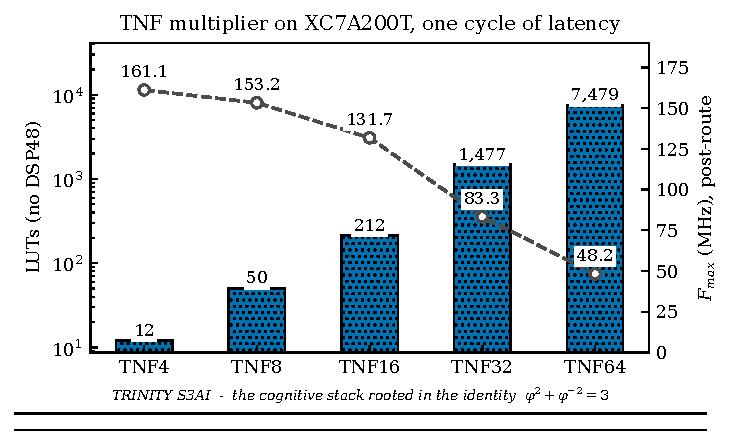
\includegraphics[width=\textwidth]{tnf_ladder.pdf}
\caption{Area and achieved frequency across the ladder.}
\label{fig:ladder}
\end{figure}

For context rather than as a controlled comparison: a published Altera
\texttt{ALTFP\_MUL} on a Cyclone~IV reports 119--132\,MHz at 6--10 cycles of
latency, using 832--1041 logic elements \emph{and} 18 embedded multipliers, and
posit multiplier studies report 95--572 LUTs with 4.28--15.55\,ns of logic delay.
Different devices and different toolchains; we draw no equivalence from them
beyond the observation that TNF16's figures sit inside that envelope on all four
axes at once, on a fabric that gives the format no ternary advantage.

Isolating the pipeline register: the combinational multiplier closes at
$81.35$\,MHz, the two-stage version at $147.32$\,MHz. The cut is between the
significand product and the renormalisation --- a $10\times10$ multiply in the
$M = 9$ module measured here, $12\times12$ at the reconciled width, then a
carry test, a saturating exponent add and a bit select.


\begin{figure}[htbp]\centering
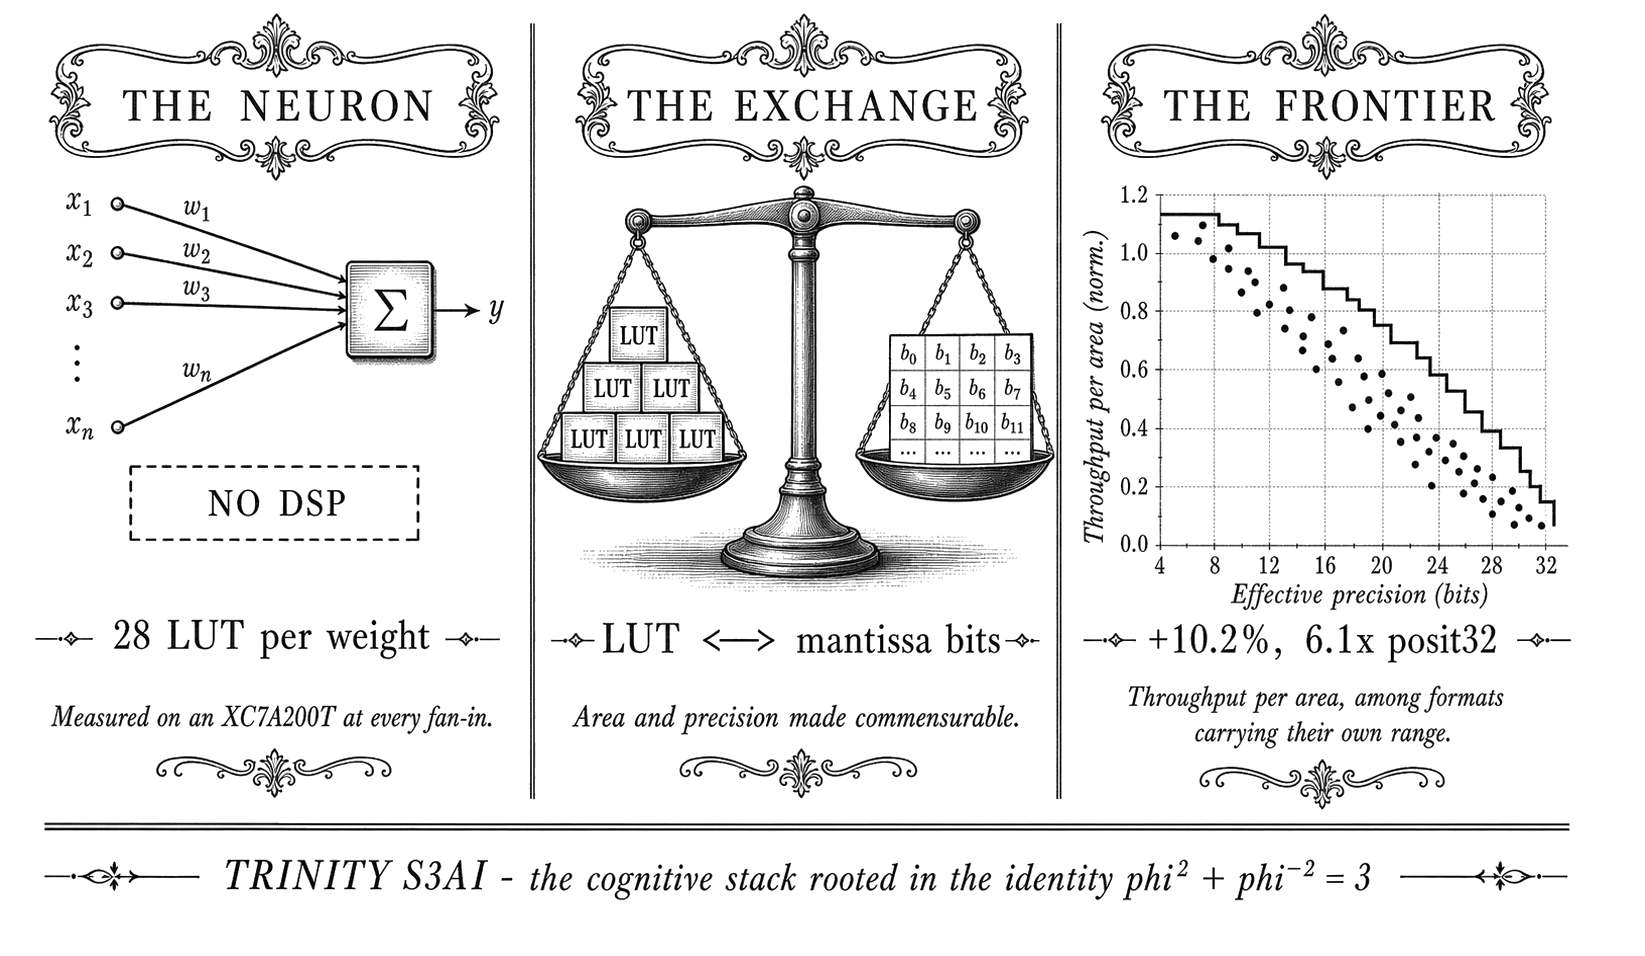
\includegraphics[width=\textwidth]{canon/canon-tnf-08-fabric.png}
\caption{What the datapath costs. The folded ternary neuron measures $28.0$ LUT per weight at fan-in $8$ and $33.1$--$33.2$ at fan-in $16$--$32$, with no DSP at any of the three, which is what makes area and precision commensurable in the fitted cost model of this section and places the format highest on throughput per LUT among the twenty-one measured formats that carry their own range.}
\label{fig:canon-fabric}
\end{figure}


% ---- tnf_paper.tex lines 1496-1658: What the law says about improving the ladder ----
\section{What the law says about improving the ladder}\label{sec:design}

\triptych{canon-tnf-22-design.png}{Packing efficiency, the log base two of three floor, and the unspent positions.}{fig:canon-design}


Theorem~\ref{thm:law} makes the design space arithmetic rather than a matter of
taste. Error scales as $2^{-(M+1)}$ and range as $3^{E_t}$, so at a fixed width
the only decision is how many bits the exponent field is allowed to consume ---
and that is decided by how efficiently $3^{E_t}$ values pack into
$\lceil E_t \log_2 3\rceil$ bits.

\begin{table}[t]\centering
\caption{Packing efficiency of the exponent field. The theoretical floor is
$\log_2 3 = 1.585$ bits per trit.}
\label{tab:pack}
\begin{tabular}{rrrrr}
\toprule
$E_t$ & values $3^{E_t}$ & bits & capacity & efficiency \\
\midrule
$3$  & $27$    & $5$  & $32$   & $84.4\%$ \\
$\mathbf{4}$  & $81$    & $7$  & $128$  & $\mathbf{63.3\%}$ \\
$5$  & $243$   & $8$  & $256$  & $\mathbf{94.9\%}$ \\
$6$  & $729$   & $10$ & $1024$ & $71.2\%$ \\
$\mathbf{7}$  & $2187$  & $12$ & $4096$ & $\mathbf{53.4\%}$ \\
$8$  & $6561$  & $13$ & $8192$ & $80.1\%$ \\
$10$ & $59049$ & $16$ & $65536$ & $90.1\%$ \\
\bottomrule
\end{tabular}
\end{table}

\paragraph{The width convention counts positions, and one rung breaks it.}
A rung's width is its position count with a trit occupying one position, so the
layout is $1 + E_t + M = N$. Three of the four specified rungs satisfy it exactly:
TNF4 is $1+2+1$, TNF8 is $1+3+4$, TNF32 is $1+6+25$. TNF16 is
$1+4+9 = 14$, two positions short of its name, and neither specification file
gives a reason. The likely history is visible in the parameters: TNF16 inherits
GF16's $\varphi$-optimal $M = 9$ and replaces GF16's six-bit exponent with four
trits, which buys range --- $3^4 = 81$ steps against $2^6 = 64$ --- and frees two
positions that were never re-spent. It is the one rung derived from its parent
rather than from the width rule.

This also settles what a rung costs on a binary fabric, which is a separate
question from its width: at the reconciled $M = 11$, a trit stored as a two-bit
code makes TNF16 twenty bits, and the offset stored as a plain binary integer
makes it nineteen --- the $18$ and $17$ of the unfilled $M = 9$ rung, which is
what the synthesised modules of \record{the full-throughput table} still carry. Those
are fabric costs, not format widths, and confusing the two is what made the
ladder appear not to fit.

\paragraph{The slack is not confined to one rung.} Applying $1 + E_t + M = N$ to
every specified rung separates the two documents that define the ladder. The four
rungs of the machine-readable specification obey it at TNF4, TNF8 and TNF32;
the five upper rungs, which exist only in a research note, miss it by four to six
positions each, and the note and the specification disagree with each other about
TNF32.

\begin{table}[t]\centering
\caption{The width rule across the ladder. $k$ is the shortfall
$N - (1 + E_t + M)$. The reconciled column is $M = N - 1 - E_t$, which changes
nothing at the three rungs that already obey the rule.}
\label{tab:ladder-sweep}
\begin{tabular}{lrrrrrr}
\toprule
rung & source & $E_t$ & $M$ & $1{+}E_t{+}M$ & $k$ & reconciled $M$ \\
\midrule
TNF4    & spec & $2$  & $1$    & $4$    & $0$ & $1$ \\
TNF8    & spec & $3$  & $4$    & $8$    & $0$ & $4$ \\
TNF16   & spec & $4$  & $9$    & $14$   & $2$ & $\mathbf{11}$ \\
TNF32   & spec & $6$  & $25$   & $32$   & $0$ & $25$ \\
TNF32   & note & $5$  & $21$   & $27$   & $5$ & --- \\
TNF64   & note & $7$  & $52$   & $60$   & $4$ & $\mathbf{56}$ \\
TNF128  & note & $8$  & $115$  & $124$  & $4$ & $\mathbf{119}$ \\
TNF256  & note & $9$  & $242$  & $252$  & $4$ & $\mathbf{246}$ \\
TNF512  & note & $10$ & $497$  & $508$  & $4$ & $\mathbf{501}$ \\
TNF1024 & note & $11$ & $1006$ & $1018$ & $6$ & $\mathbf{1012}$ \\
\bottomrule
\end{tabular}
\end{table}

No single alternative convention explains the upper rungs either: reading the
exponent as $\lfloor E_t\log_2 3\rfloor$ bits fits TNF16, TNF64, TNF128 and
TNF1024 exactly but overshoots TNF256 and TNF512 by one and misses TNF32
entirely. We conclude that the upper ladder was tabulated rung by rung rather than
derived, and that reconciling it costs nothing at the rungs that are already
right.

\paragraph{What the two free positions were worth, and where they went.} Because
the exponent cancels in Theorem~\ref{thm:law}, the menu at sixteen positions could
be read off before measuring, and the measurement confirmed it to four significant
figures:

\begin{table}[t]\centering
\caption{The three ways to spend TNF16's two unallocated positions, on the
harness of Table~\ref{tab:acc}: mean relative error in the far band, $|e|$ in
$[20,38)$, no row overflowing. Error and range trade against each other exactly
as Theorem~\ref{thm:law} predicts; nothing in any row is worse than the unfilled
rung. The published version of this table read $3.37\mathrm{e}{-4}$,
$8.63\mathrm{e}{-5}$ and $5.46\times$ from an earlier harness, which is why it did
not agree with the accuracy table a few pages earlier. The \emph{positions} column
is the nominal budget of Section~\ref{sec:budget}: the adopted rung occupies
$1+\lceil 4\log_2 3\rceil+11=19$ physical cells and the two $E_t{=}5,6$ variants
occupy $20$ and $22$. \record{The applicability section} measures what happens when the
comparison is held to sixteen cells instead.}
\label{tab:tnf16-fill}
\begin{tabular}{lrrrr}
\toprule
variant & positions & mean rel.\ error & decades & vs.\ takum16 (far) \\
\midrule
unfilled, $E_t{=}4$, $M{=}9$  & $14$ & $3.39\mathrm{e}{-4}$ & $24$  & $5.66\times$ \\
$\mathbf{E_t{=}4}$, $\mathbf{M{=}11}$ (adopted) & $\mathbf{16}$ & $\mathbf{8.45\mathrm{e}{-5}}$ & $24$ & $\mathbf{22.68\times}$ \\
$E_t{=}5$, $M{=}10$           & $16$ & $1.72\mathrm{e}{-4}$ & $73$  & $11.14\times$ \\
$E_t{=}6$, $M{=}9$            & $16$ & $3.39\mathrm{e}{-4}$ & $\mathbf{219}$ & $5.66\times$ \\
\bottomrule
\end{tabular}
\end{table}

The last row is the law's own consistency check: adding two trits of exponent
while holding $M$ leaves the error bit-identical and multiplies the range
ninefold.

\paragraph{The positions were spent on mantissa, and the reason is a measurement.}
\record{the three-currencies corollary} forbids recommending a budget without naming a workload,
so we named one. At the 16-bit class the extra range is not consumed:
quantised-inference tensors span roughly $2^{-14}$ to $2^{14}$, and $E_t = 4$
already clips nothing at $\pm 39$ binades --- zero clips in 2000 values. $E_t = 6$
would have bought $\pm 363$ binades at bit-identical error, which is range nobody
spends at sixteen bits. So $M = 11$: the error falls by $4.09$, which is what two
more mantissa bits buy, and against takum16 the rung moves from
$0.90\times / 2.72\times / 5.66\times$ to $3.70\times / 11.21\times / 22.68\times$,
no longer losing the near bin. Both figures are at the nominal budget, where this
rung is a nineteen-cell object compared against a sixteen-cell one; held to
sixteen cells it loses the near bin again, at $0.46\times$
(\companion{the equal-storage accuracy table}), and it loses to \texttt{binary16} everywhere
(\record{the crossover-window table}). On the XC7A200T it costs $443$ LUTs against $372$,
a $19\%$ increase, at $136.44$\,MHz against $131.73$ --- no frequency penalty.

All three ratios in this section and in Figure~\ref{fig:acc} come from one
script, \texttt{gen\_figures.py}, which computes them from the oracles at seed
$20260809$ rather than transcribing them. They were hardcoded until 2026-08-09 and
had drifted: the figure still carried $M = 9$ and the label \texttt{tekum16} after
the rung moved and the oracle was shown to decode identically to takum. A figure
that disagrees with the table it illustrates is the same defect class as a gate
that cannot go red.

Conformance was re-run in full rather than assumed: round-trip with sign
2000/2000, encoding monotone with zero inversions, $\pm$ symmetry with zero
mismatches in 500, both range boundaries decoding. A \texttt{width\_rule} test now
asserts $1 + E_t + M = N$ in the specification itself, so the position count is
checked rather than remembered. All nine rungs satisfy it \emph{as reconciled} ---
that is, at the $M$ values in the last column of Table~\ref{tab:ladder-sweep}. Five
upper rungs satisfy it only there and not in the research note they come from, and
no hardware has been placed at those reconciled widths.
\triptych{canon-tnf-61-audittrail.png}{After the TNF16 reconciliation, the paper records a stale generated figure, reruns full conformance, and puts the width rule into the specification as an assertion.}{fig:canon-b4-61audittrail}



% ---- tnf_paper.tex lines 1659-2046: Why ternary, and exactly how much ----
\section{Why ternary, and exactly how much}\label{sec:whyternary}

\triptych{canon-tnf-13-whyternary.png}{The ternary case of this section, bounded in both directions: radix economy as a state-slot argument, what a binary fabric takes back from the encoding, and the separation of the radix choice from the encoding.}{fig:canon-whyternary}


The case for a ternary exponent is usually made by citing radix economy and left
there. We state it, then bound it in two directions --- what a binary fabric takes
back, and what the radix of the \emph{scale} is worth as distinct from the radix
of the \emph{exponent} --- because both bounds turn out to be decisive for the
design and neither is folklore.

\begin{theorem}[Radix economy]
\label{thm:economy}
Representing $R$ distinct values in radix $b$ costs $b\log_b R = b\ln R/\ln b$
state-slots. The factor $b/\ln b$ is minimised at $b = e$; among integers it is
$3/\ln 3 = 2.731$ against $2/\ln 2 = 2.885$, so a ternary field is $5.4\%$ more
economical than a binary one \emph{in state-slots}. The qualifier is not a
formality: \companion{the range-per-bit theorem} shows the advantage does not survive
re-expression in binary cells, and no result in this paper asserts it there.
\end{theorem}

\begin{proof}
A radix-$b$ numeral addressing $R$ values needs $\log_b R$ digit positions, and a
position that must hold any of $b$ symbols costs $b$ state-slots, giving
$C(b) = b\log_b R = (b/\ln b)\ln R$. Since $\ln R$ is a positive constant in $b$,
minimising $C$ is minimising $g(b) = b/\ln b$. Then
$g'(b) = (\ln b - 1)/\ln^{2} b$, which is negative for $1 < b < e$, zero at
$b = e$ and positive for $b > e$, so $g$ has its unique minimum at $b = e$ and is
strictly increasing above it. Among integers the candidates are therefore $2$ and
$3$, the two neighbours of $e = 2.71828$, and $g(3) = 2.73072 < g(2) = 2.88539$.
The relative saving is $1 - g(3)/g(2) = 0.05361$.
\end{proof}

This is the classical argument~\cite{hayes2001,radixeconomy} and it is what
motivates a ternary exponent. It is also stated in a currency --- state-slots ---
that no binary fabric pays in. The next theorem says what happens when it does.

The classical argument also has a published rebuttal, and this paper's position is
that the rebuttal is correct on its own terms. Etiemble argues that $R=3$ is
\emph{not} the optimal radix for computation~\cite{etiemble2019}: once the metric
is switched from abstract state-slots to the delay, area and energy of a realised
ternary gate on a binary-optimised process, the $5.4\%$ slot advantage is consumed
several times over. Nothing in this paper contradicts that. The $5.4\%$ is quoted
here as the classical statement being bounded, not as a design justification, and
Theorem~\ref{thm:nofree} together with Theorem~\ref{thm:packing-density} is
precisely the statement that it is never collected on the fabric this work uses.
The ternary field is adopted because the exponent field is a \emph{value-set}
question --- a balanced alphabet $\{-1,0,+1\}$ makes the sign a select rather than
a branch, per Section~\ref{sec:closure} --- and not because three is the optimal
radix for computation. Any claim of the latter kind should be read as refuted by
Etiemble's argument [refuted --- external].

A radix argument for the exponent field is also not unique to three. The
AetherFloat family~\cite{aetherfloat} proposes block-scale-free \emph{quad}-radix
floating-point for AI accelerators, occupying the same design slot --- a
non-binary base in the scale --- from radix four. The distinction is not which
radix is better in the abstract, which by Etiemble's argument is the wrong
question. It is that a radix of the form $2^{k}$ keeps the scale a shift, which is
the content of \record{the optimal-radix theorem}, so radix four buys its non-binary block
structure while staying multiplier-free on a binary datapath; radix three does
not, and the datapath of Section~\ref{sec:closure} is what pays for it. Both
positions are coherent and they are not interchangeable, and this paper makes no
claim of superiority over the quad-radix route [open].

\begin{theorem}[No free range on a binary fabric]
\label{thm:nofree}
An exponent field of $E_t$ trits spans $3^{E_t}$ values. Stored as a binary
integer it occupies $\lceil E_t\log_2 3\rceil$ bits, a field spanning
$2^{\lceil E_t\log_2 3\rceil} \geq 3^{E_t}$ values. Hence on a binary fabric a
ternary exponent never spans more values per bit than a binary one, with equality
only at $E_t = 0$. Writing $\rho(E_t) = 3^{E_t}/2^{\lceil E_t\log_2 3\rceil}$ for
the utilisation, $\rho \in (1/2, 1]$ and $\rho$ does not converge.
\end{theorem}
\begin{proof}
The ceiling gives $2^{\lceil E_t\log_2 3\rceil}\geq3^{E_t}$.  For
$E_t>0$ equality would imply $3^{E_t}=2^q$ for an integer $q$, which is
impossible by unique factorisation; at $E_t=0$ both sides are one.  For
$E_t>0$, the fractional part of $E_t\log_2 3$ is non-zero and
$\rho(E_t)=2^{\{E_t\log_2 3\}-1}$, hence $\rho(E_t)\in(1/2,1)$.  The number
$\log_2 3$ is irrational, so its positive integer multiples have dense
fractional parts in $(0,1)$; the displayed continuous map consequently has
subsequences approaching both endpoints, and $\rho$ cannot converge.
\end{proof}

\begin{table}[t]\centering
\caption{Utilisation $\rho(E_t)$ of the binary field holding an $E_t$-trit
exponent. $E_t = 7$, a budget the ladder uses, is the worst entry in the range at
$53.4\%$; $E_t = 4$ at $63.3\%$ is a low entry but not the second worst, which is
$E_t = 2$ at $56.2\%$.}
\label{tab:rho}
\begin{tabular}{lrrrrrrrrrr}
\toprule
$E_t$ & 2 & 3 & 4 & 5 & 6 & 7 & 8 & 9 & 10 & 11 \\
\midrule
$\rho$ & $56.2$ & $84.4$ & $\mathbf{63.3}$ & $94.9$ & $71.2$ & $\mathbf{53.4}$ & $80.1$ & $60.1$ & $90.1$ & $67.6$ \\
\bottomrule
\end{tabular}
\end{table}

Run as an optimisation rather than an inequality, the same statement is sharper
than it looks. Asking which exponent encoding a binary fabric prefers at
$(N, R) = (16, 24)$, $(32, 219)$ and $(64, 658)$ --- the decade counts of
$E_t = 4$, $6$ and $7$; the shipped ladder uses $E_t = 5$ at 32 bits and so spans
$73$ decades there --- returns the same mantissa width
for both --- $M = 10$, $23$ and $53$ respectively. The ternary encoding does not
lose on a binary fabric; at these widths the ceilings absorb the difference and it
exactly ties, which is the strongest form of ``never more values per bit''.

Theorem~\ref{thm:nofree} is the reason the ladder's rung widths must be read as
position counts and not bit counts, and it is where our own first reading of the
ladder went wrong: measuring what a trit costs when packed into bits and calling
the result the format's width confuses a fabric cost with a format property. The
independently published balanced-ternary float Ternary27~\cite{ternary27} counts
the same way --- 2 type trits, 1 sign trit, 5 exponent trits and 19 significand
trits, exactly 27 --- which is external corroboration that position counting is
the convention in this family rather than a reading of our own.

The loss in Theorem~\ref{thm:nofree} is not only non-zero; it has a rigid
arithmetic shape, and the utilisation it leaves behind is not eventually
well-behaved.

\begin{theorem}[The binary-packing loss has a dense utilisation spectrum]
\label{thm:packing-density}
For $t\geq1$ put $b_t=\lceil t\log_2 3\rceil$, $L_t=2^{b_t}-3^{t}$ and
$\rho_t=3^{t}/2^{b_t}$. Then $L_t$ is a positive odd integer. Moreover
$\{\rho_t : t\geq1\}$ is dense in $(1/2,1)$, so its set of limit points is
$[1/2,1]$.
\end{theorem}
\begin{proof}
$2^{b_t}$ is even and $3^{t}$ is odd, so they are never equal and $L_t$ is odd;
$L_t>0$ by the definition of the ceiling. Next, $\log_2 3$ is irrational, since
$\log_2 3=p/q$ would give $3^{q}=2^{p}$. Hence $\{t\log_2 3\}$ is
equidistributed, and therefore dense, in $(0,1)$, and
$\rho_t=2^{\{t\log_2 3\}-1}$. The map $x\mapsto2^{x-1}$ is a continuous
increasing bijection from $(0,1)$ onto $(1/2,1)$, which transports density.
\end{proof}

Checked as exact integers for $t=1,\dots,500$: $L_t>0$ and odd in every case,
beginning $(t,b_t,L_t)=(1,2,1)$, $(2,4,7)$, $(3,5,5)$ and reaching
$L_{16}=24{,}062{,}143$ at $b_{16}=26$. Two readings follow. There is no trit
budget at which binary packing is free, so the ``$5.4\%$ more economical'' of
Theorem~\ref{thm:economy} is never collected on a binary fabric. And because the
utilisation is dense in $(1/2,1)$, no tail of the ladder is asymptotically safe:
Table~\ref{tab:rho} is a sample of a sequence with limit points filling the whole
interval, which is why the rung-by-rung figure has to be quoted rather than a
limit.

\begin{theorem}[Unallocated positions are a pure loss]
\label{thm:alloc}
Let a rung of $N$ positions carry a sign, $E_t$ exponent trits and $M$ mantissa
bits with $1 + E_t + M = N - k$, $k \geq 0$. Then relative to the rung with the
same $E_t$ and $M + k$, its expected relative error is larger by exactly $2^{k}$
and its dynamic range is identical.
\end{theorem}

\begin{proof}
By Theorem~\ref{thm:law} the expected relative error is
$\tfrac12 \mathbb{E}[1/s]\,2^{-(M+1)}$, in which the exponent does not appear;
replacing $M$ by $M+k$ multiplies it by $2^{-k}$. The dynamic range is
$3^{E_t}-2$ binades, a function of $E_t$ alone, so it is unchanged. Nothing else in
the layout depends on $M$.
\end{proof}

Theorem~\ref{thm:alloc} converts the slack of Section~\ref{sec:design} into a
number without any measurement, and the measurement then confirms it. Against a
workload built in exact arithmetic --- necessary above TNF32, where a
double-precision probe measures its own resolution rather than the format's ---
the predicted and observed factors are:

\begin{table}[t]\centering
\caption{Unallocated positions per rung, the loss Theorem~\ref{thm:alloc}
predicts, and the loss measured against the reconciled rung
$M = N - 1 - E_t$. Exact-arithmetic workload, 800 probes per rung.}
\label{tab:alloc}
\begin{tabular}{lrrrr}
\toprule
rung & $k$ & predicted & measured \\
\midrule
TNF16  & $2$ & $4\times$  & $4.03\times$  \\
TNF64  & $4$ & $16\times$ & $15.43\times$ \\
TNF128 & $4$ & $16\times$ & $15.99\times$ \\
TNF256 & $4$ & $16\times$ & $15.24\times$ \\
\bottomrule
\end{tabular}
\end{table}

The final question is one the ladder answers implicitly and, as far as we can
find, no one has stated: TNF encodes its exponent in radix 3 but scales by
$2^{e}$, whereas Ternary27 scales by $3^{e}$. These are different choices and
they are separable.

\begin{theorem}[Scale radix: under the log-uniform model at fixed field layout,
$r=2$ has lower relative error than $r=3$]
\label{thm:scaleradix}
Let a format scale by $r^{e}$ with a normalised significand uniformly quantised
over $[1, r)$ by $M$ bits. Then its expected relative error on a log-uniform
workload is $\tfrac14\kappa(r)\,2^{-M}$ with
\[
\kappa(r) \;=\; \frac{(r-1)^{2}}{r\ln r},
\qquad \kappa(2) = 0.72135,\quad \kappa(3) = 1.21365 .
\]
Holding the field layout fixed, moving the scale from $r=2$ to $r=3$ therefore
multiplies the error by $\kappa(3)/\kappa(2) = 1.6825$ while multiplying the
dynamic range by $\log_2 3 = 1.5850$. Measured in positions, it costs
$\log_2 1.6825 = 0.7506$ of precision and buys $\log_3 1.5850 = 0.4192$ of range:
a net loss of $0.3314$ positions per number. Under this model, and counting in
abstract radix positions rather than in packed binary storage, a power-of-two
scale therefore has the lower predicted error at equal position count. The
comparison is not a statement about packed width on a binary fabric: by
Theorem~\ref{thm:nofree} a trit-indexed field must additionally pay
$\lceil E_t\log_2 3\rceil$ bits of storage, and that cost is accounted separately
in \record{the boundary theorem}.
\end{theorem}

\begin{proof}
The quantisation step over $[1,r)$ is $\Delta = (r-1)2^{-M}$. Under
round-to-nearest the signed error is uniform on $(-\Delta/2, \Delta/2)$, so the
mean \emph{absolute} error is $\Delta/4$ --- a quarter of the step, not half of
it, which is the maximum rather than the mean. On a log-uniform workload the
significand has density $1/(s\ln r)$ on $[1,r)$, so
$\mathbb{E}[1/s] = \frac{1}{\ln r}\int_1^{r} s^{-2}\,ds = \frac{1-1/r}{\ln r}$.
Multiplying gives $\tfrac14 (r-1)2^{-M}\cdot\frac{1-1/r}{\ln r}$, and
$(r-1)(1-1/r) = (r-1)^2/r$, which is $\tfrac14\kappa(r)2^{-M}$ as stated. For
the range, $E_t$ trits span $3^{E_t}$ exponent states --- $3^{E_t}-2$ of them
ordinary in TNF, the two extremes being reserved --- of $\log_2 r$ binades each. One
mantissa bit halves the error and one exponent trit triples the range, which
fixes the exchange rate between the two currencies and gives the position
figures.
\end{proof}

Direct measurement at two rungs, encoding and decoding through both scales in
exact arithmetic, gives error ratios of $1.675$ at $(E_t,M) = (4,11)$ and $1.690$
at $(6,25)$ against the predicted $1.6825$, and range ratios of $1.583$ and
$1.585$ against the predicted $1.5850$.

\paragraph{The prefactor was wrong by a factor of four, and only the prefactor.}
An earlier statement of this theorem gave the expected error as $\kappa(r)2^{-M}$,
because the proof took the mean rounding error to be half a step rather than a
quarter and then absorbed a second factor of two into a convention. A Monte-Carlo
check of $8\times10^{6}$ log-uniform draws returns $7.0471\times10^{-4}$ at
$(r,M)=(2,8)$ against $\tfrac14\kappa(2)2^{-8} = 7.0444\times10^{-4}$, and
$1.4822\times10^{-4}$ at $(3,11)$ against $\tfrac14\kappa(3)2^{-11} =
1.4815\times10^{-4}$, so the corrected prefactor is confirmed to four figures
\textbf{[measured --- software]}. Nothing downstream moves: every use of $\kappa$
elsewhere in this paper is a \emph{ratio}, and $\kappa(3)/\kappa(2) = 1.6825$ is
unchanged by a common factor, as is the minimisation of $\kappa$ over the
shift-only set in \record{the optimal-radix theorem}. This is recorded rather than
silently corrected because an absolute constant that no ratio depends on is
exactly the kind of number a reader will lift out of context.

\begin{corollary}[What TNF is, precisely]
TNF is not a ternary float in the sense of Ternary27; it is a binary-radix float
whose exponent is \emph{encoded} in balanced ternary. Theorem~\ref{thm:scaleradix}
says that under its log-uniform, fixed-layout model this choice has the lower
predicted relative error of the two available ones, by $0.331$
position-equivalents per number, and Theorem~\ref{thm:nofree} says that the ternary encoding pays only on a
ternary fabric. The two together delimit the format exactly: the radix choice is
right on any fabric, and the encoding choice is right on one.
\end{corollary}
\triptych{canon-tnf-59-stateslotledger.png}{Ternary is more economical in state-slots, but binary packing restores the cost and yields equal mantissa widths in the named tested cases.}{fig:canon-b4-59stateslotledger}



\subsection{A 27-level element on a trit substrate, measured}
\label{sec:t27block}

The corollary above says where the encoding choice pays: on a fabric whose
storage cell is physically ternary. \record{The block-axis section} measured
shared-scale blocks on binary storage, and there the formats of this paper
lose. What neither settles is what a \emph{block} format
gains when a position is a trit, the one setting in which
\record{the slack-artefact corollary} says the slack survives. This subsection
answers that with one pre-registered measurement. The answer is the slack of
that corollary, measured on a language model; it is not a new advantage, and
the bit-axis reading below says why.

\paragraph{The element.} A three-trit cell holds $27$ codes. The element here,
called T27, spends all of them: zero and $13$ symmetric magnitudes, with one
power-of-two scale per block of $32$ weights stored in $5$ trits. The magnitudes
are the NF4 construction~\cite{qlora} carried to $27$ levels: the $k$-th is
$\Phi^{-1}(p_k)/\Phi^{-1}(p_{13})$ with $p$ spaced evenly on
$[\tfrac12,\tfrac{53}{54}]$, rounded to $1/1024$, which gives
$\{0,46,92,139,187,237,289,346,407,475,554,651,782,1024\}/1024$. T27 is a
codebook, not a TNF rung: it has no exponent field, and it is not TNF4\_7, which
gives $36.76$ on the same run.

\paragraph{What was fixed before the run.} The specification
\texttt{specs/\allowbreak numeric/\allowbreak ternary\_\allowbreak storage\_\allowbreak search\_\allowbreak v2.t27} (sha256 prefix
\texttt{88fcf517}) was committed at \texttt{49a84ade5} before any arm ran. It
compiles under the t27 compiler, its test blocks pass, and it generates the
runner's parameters, so the runner cannot hold a number the specification does
not. It fixes the formats, the storage count and a verdict ladder.
\begin{itemize}
\item Storage: on a trit substrate each field takes the fewest trits that hold
  its codes. Per $32$ weights this gives T27 $101$, MXFP4 $102$, MX+ $106$,
  NVFP4 $106$ and the five-bit binary element E2M2 $134$.
\item Ladder: for each comparator $C$, $r = 1000\cdot\mathrm{ppl(T27)}/\mathrm{ppl}(C)$.
  $r\le 990$ reads ``T27 better'', $r\le 1010$ a tie, anything above ``$C$
  better''. NVFP4~\cite{nvfp4} is the primary comparator; MX+~\cite{mxplus} and
  MXFP4 are read on the same ladder.
\item Selection: three 27-level candidates, one chosen on the validation split
  (the normal-quantile one, $16.6880$). The test split was read once, after the
  choice.
\item Rulers: the unquantised model, MXFP4 and TNF4\_7 had to reproduce a first
  attempt's numbers on the same machine within $0.001$. They reproduced to
  $0.0000$. The first attempt had stopped at its own ruler stage, because
  TNF4\_7 differed from another machine's value by $0.0398$ against a tolerance
  of $0.01$; no arm of it ran.
\end{itemize}

\begin{table}[t]\centering
\caption{SmolLM2-135M, wikitext-2 test, $40$ windows of $2048$ tokens, weights
only, one run per arm. The trit column is the pre-registered axis; the bit
column is shown for comparison and is read below. NVFP4 adds $32$ bits per
tensor. $r$ is the ladder value against T27, in per mille.}
\label{tab:t27block}
\begin{tabular}{lrrrrr}
\toprule
element & ppl & $\times$ \texttt{fp32} & trits/32 & bits/32 & $r$ \\
\midrule
unquantised                  & $14.4869$ & $1.000$ & ---   & ---        & ---     \\
E2M2 (5-bit binary)          & $15.8083$ & $1.091$ & $134$ & $168$      & ---     \\
\textbf{T27}                 & $\mathbf{16.2892}$ & $1.124$ & $\mathbf{101}$ & $161$ dense & ---     \\
NVFP4                        & $17.4697$ & $1.206$ & $106$ & $144$      & $932.4$ \\
MX+                          & $17.9780$ & $1.241$ & $106$ & $141$      & $906.1$ \\
MXFP4 (E2M1)                 & $21.9353$ & $1.514$ & $102$ & $136$      & $742.6$ \\
\bottomrule
\end{tabular}
\end{table}

\paragraph{What was measured.} Every verdict on the ladder is ``T27 better''
(Table~\ref{tab:t27block}): $932.4$ against NVFP4, $906.1$ against MX+ and
$742.6$ against MXFP4 on test, and $926.0$, $907.9$ and $737.5$ on the
validation split. T27 does it in $101$ trits per $32$ weights against $106$,
$106$ and $102$, and closes $40\%$ of NVFP4's excess perplexity over the
unquantised model ($1.80$ against $2.98$) \textbf{[measured --- software]}. The
three predictions written into the specification held, one of them that E2M2
would do at least as well as T27, and so did the author's guess recorded beside
them as a guess. The mechanism is the one the specification
gave in advance. E2M1 fills $16$ of the $27$ codes a three-trit cell holds, and
T27 fills all of them, which is $\log_2(27/16)=0.75$ bit more code per
element; that outweighs NVFP4's finer scale, one E4M3 value per $16$ weights
where T27 has one power of two per $32$.

\paragraph{The same numbers in bits.} This reading is post hoc and is labelled
so. Packed densely on binary memory, T27 costs $\lceil 101\log_2 3\rceil=161$ bits per $32$
weights, against $144$ for NVFP4, and E2M2 at $168$ bits beats it. The straight line between
NVFP4 and E2M2 predicts $16.2929$ at $161$ bits; T27 measures $16.2892$, $0.0037$ below the
chord. If the binary frontier is convex between those two points, which is the usual shape and
was not measured here, it lies on or below that chord, so on binary memory T27 beats it by at
most $0.0037$: level with formats that already exist. That is \record{the slack-artefact corollary}
observed in perplexity. The corollary is stated for an exponent field and T27 has none, but its
proof counts only trits against the bits that hold them, and that count is the same here: the
advantage is real on the position axis and disappears on the bit axis (Theorem~\ref{thm:nofree}).

\paragraph{What it would take in silicon.} Per $32$ weights T27 needs $101$ trit
cells where NVFP4 needs $144$ bit cells. T27 is the smaller store only if one
trit cell costs less than $144/101=1.43$ bit cells, which is $0.90$ of the
$\log_2 3=1.585$ bits of information the cell carries; against MX+ the bound is
$1.40$. The ternary compute-in-memory literature stores a trit in two binary
cells and argues that native three-state cells are harder to read
reliably~\cite{retern}. At two cells per trit T27 needs $202$ bit cells, and
NVFP4 is the smaller store. The result therefore names a condition on the cell,
not a win: a native ternary cell costing under $1.43$ bit cells.

\paragraph{What it does not say.} It covers one model, one corpus and weights
only; activations and the KV cache were not touched. It has no uncertainty
interval: the ladder is a point comparison on $40$ windows, a per-window paired
bootstrap was not pre-registered, and none is claimed. The margins are large
against a $990$ bar, but that is judgement, not a test. NVFP4 and MX+ are
re-implementations, of NVIDIA's published two-level weight recipe and of the
MX+ paper's description, not of the authors' code; MX+ uses the OCP scale rule
$\lfloor\log_2 a_{\max}\rfloor-2$. The MXFP4 row uses the first attempt's
ceiling E8M0 scale on this machine. It is not to be read across into
\record{the block-axis table}, which reports $22.4998$ for MXFP4 from another
script on another machine; that difference is not resolved here. The record
is \texttt{research/\allowbreak block/\allowbreak TERNARY\_\allowbreak STORAGE\_\allowbreak V2\_\allowbreak VERDICT\_\allowbreak 2026-09-27.md}, at
commit \texttt{d31d8523c}.



% ---- tnf_paper.tex lines 3605-3893: Two formats close a ternary node ----
\section{Two formats close a ternary node}\label{sec:pair}

\triptych{canon-tnf-26-pair.png}{Three sites, the forced alphabet, and what depth costs.}{fig:canon-pair}


A ternary node contains exactly three sites where a number format could live, and
only one of them needs one.

\begin{enumerate}
\item The \textbf{weight} is a code. Multiplying by it is a sign-select
      ($+x$, $-x$, $0$), not a multiply.
\item The \textbf{sample} arrives ADC-native and is used as it lands.
\item The \textbf{accumulator} is the only object in the system carrying a
      dynamic range that must be spent.
\end{enumerate}

This is the whole design problem, and it is smaller than the literature makes it
look. The published ternary methods answer (1) and leave (3) in \texttt{fp16} or
\texttt{int8}; the published format work answers (3) and assumes a multiplier at
(1). We answer both, with two formats that were derived independently and turn
out to be complements.

\subsection{Why the weight alphabet is \texorpdfstring{$\varphi$}{phi}, and why that is forced}
\triptych{canon-tnf-40-phialphabet.png}{Closure under multiplication forces the quadratic whose positive root is the base, so the inter-layer gain is a pair of integers rather than a learned scale.}{fig:canon-phialphabet}


GFTernary is a two-bit alphabet $\{-\varphi,\,0,\,+\varphi\}$. The $\varphi$ is
not decoration, and the following says why it is the only choice inside the
class of alphabets the datapath's own additive lattice can close over.

\begin{theorem}[Uniqueness of the golden alphabet within the lattice-closure
class]
\label{thm:goldalpha}
Let a three-symbol weight alphabet be $\{-r,0,+r\}$ with $r>1$, and require that
the product of two weights be expressible in the additive lattice the datapath
already computes in, i.e.\ $r^2 = r + 1$. Then $r = \varphi$ uniquely.
\end{theorem}
\begin{proof}
$r^2 - r - 1 = 0$ has roots $(1\pm\sqrt5)/2$, of which one is positive.
\end{proof}

\begin{corollary}[Depth costs no multiplier]
\label{cor:depth}
The gain of a stack of $k$ ternary $\varphi$-layers is exactly
\[
  \varphi^{k} = F_k\,\varphi + F_{k-1},
\]
a pair of integers with $F$ the Fibonacci sequence. Rescaling between layers is
therefore a shift-and-add, and the zero-multiplier property survives to arbitrary
depth.
\end{corollary}
\begin{proof}
For $k=1$ the identity is $\varphi=F_1\varphi+F_0$. If
$\varphi^k=F_k\varphi+F_{k-1}$, multiplication by $\varphi$ and
$\varphi^2=\varphi+1$ give
$\varphi^{k+1}=F_k+ (F_k+F_{k-1})\varphi
=F_{k+1}\varphi+F_k$.
Induction proves the identity for every $k\geq1$. The coefficients are integers,
so multiplying a lattice pair by $\varphi$ is the map $(a,b)\mapsto(b,a+b)$,
which is a shift-and-add operation and introduces no multiplier.
\end{proof}

This is the practical content of Theorem~\ref{thm:goldalpha}, and it is what
separates the $\varphi$ alphabet from the $\{-1,0,+1\}$ one used throughout the
ternary-network literature. With unit weights the layer gain is $1$ and carries no
information, so every published method attaches a learned real scale $\alpha_\ell$
per layer --- and multiplying by $\alpha_\ell$ puts the multiplier back. With the
$\varphi$ alphabet the inter-layer scale is known exactly and is a pair of
integers, so it is never multiplied by. Storage is two bits either way and the
symbol count is three either way; the $\varphi$ alphabet simply carries a scale
that the unit alphabet has to learn and then pay for.


\subsection{The linear path is exact}
\triptych{canon-tnf-41-exactlinear.png}{The accumulator carries two integers, multiplication by the base is a relabelling plus one addition, and a fan-in of 512 costs eight bits per component.}{fig:canon-exactlinear}

\label{sec:exact}

Theorem~\ref{thm:goldalpha} is usually read as removing a multiplier. It removes
the rounding with it: on the alphabet it fixes, the entire linear path of a
network is computed exactly.

Represent a value as an integer pair $(a,b)$ standing for $a + b\varphi$. Then
\[
  \varphi\,(a + b\varphi) \;=\; a\varphi + b\varphi^{2} \;=\; a\varphi + b(\varphi+1)
  \;=\; b + (a+b)\varphi ,
\]
so applying a weight is the map $(a,b) \mapsto (b,\,a+b)$ --- the Fibonacci
recurrence, one integer addition, no shift. Negation flips both components and a
zero weight is a skip.

\begin{theorem}[Exactness of the multiply-free path]
\label{thm:exact}
$\mathbb{Z}[\varphi] = \{a + b\varphi : a,b \in \mathbb{Z}\}$ is a ring, and the
weight alphabet $\{-\varphi,0,+\varphi\}$ lies inside it. Hence for inputs in
$\mathbb{Z}[\varphi]$ the entire linear part of a ternary network --- every
weight application and every accumulation, to arbitrary fan-in and arbitrary
depth --- remains in $\mathbb{Z}[\varphi]$ and is computed \emph{without
rounding error of any kind}.
\end{theorem}
\begin{proof}
Closure under addition is componentwise. Closure under multiplication follows
from $\varphi^2 = \varphi + 1$, which reduces every product to the stated
integer-pair map. The accumulator is therefore a pair of exact integer registers.
\end{proof}

Measured on a layer of fan-in $512$ with weights drawn from the alphabet, the
integer pair reproduces the real-valued sum to the precision of the checking
arithmetic and not to the precision of the datapath: there is nothing in the
datapath to be imprecise. The component widths grow logarithmically, reaching
eight bits over those $512$ terms.

Closure gives exactness of the path. The next statement gives something narrower
but more useful in a test harness: a check on the composed layer gains that runs
in integers only, so that a conformance test for the depth-$k$ path needs no
floating point at all.

\begin{theorem}[Even-power Lucas trace certificate]
\label{thm:lucas-trace}
For every integer $n\geq0$,
\[
 \varphi^{2n}+\varphi^{-2n}=L_{2n}\in\mathbb{Z},
\]
and these values are generated exactly in integer arithmetic by $S_0=2$,
$S_1=3$, $S_{n+2}=3S_{n+1}-S_n$.
\end{theorem}
\begin{proof}
The conjugate of $\varphi$ is $\bar\varphi=1-\varphi=-\varphi^{-1}$, so
$\varphi^{2n}+\varphi^{-2n}=\varphi^{2n}+\bar\varphi^{2n}$, the trace of the
algebraic integer $\varphi^{2n}$, which Binet's formula identifies with $L_{2n}$.
Both $\varphi^{2}$ and $\bar\varphi^{2}$ are roots of $x^{2}-3x+1=0$, and the
trace sequence of a quadratic satisfies the recurrence read off its coefficients.
\end{proof}

The $n=1$ case is the identity $\varphi^{2}+\varphi^{-2}=3$ that gives this work
its name; the theorem is the statement that the identity is the first term of an
integer sequence rather than a coincidence at one exponent. The recurrence and the
Lucas definition agreed at every $n=0,\dots,256$ in Python integers, with
$L_0,L_2,L_4,L_{10}=2,3,7,123$. What it licenses is a test, not a claim about
accuracy: a depth-$k$ $\varphi$-stack can be audited against
$S_k$ with no rounding model in the loop, which is the property
Corollary~\ref{cor:depth} needs in order to be checkable on hardware. It says
nothing about downstream model quality [proved --- exact integer arithmetic].

\subsection{Closure is what removes the machinery}\label{sec:closure}

The multiply-free datapath is not new as an aim, and the published attempts make
the role of Theorem~\ref{thm:exact} visible by contrast.

The closest is FQP~\cite{fqp}, a Fibonacci quantization processor that turns the
products of Fibonacci-quantized weights into additions. To do so it carries two
distinct arithmetic units --- a dualistic-transformation adder for the large
operands and a bit-exclusive adder for the small ones --- and a topological-order
routing scheme that maps data onto them. Fibbinary quantization for neural radio
receivers~\cite{fibbinary} takes the softer route on the same substrate and
reports $45\%$ and $44\%$ savings in multiplier power and area: the multiplier is
made cheaper, not removed.

The machinery in the first is not an artefact of implementation. It follows from
a property of the number set.

\begin{corollary}[Closure removes the transformation stage]\label{cor:closure}
Let $A$ be a weight alphabet and let $s$ be the operation that applies a weight.
If the additive group generated by $A$ is closed under $s$, the datapath needs
only that group's addition. If it is not, every product must be re-expressed in
the representable set, which requires a transformation stage and a schedule that
routes operands to it.
\end{corollary}
\begin{proof}
Immediate from Theorem~\ref{thm:exact} and its negation. For
$A=\{-\varphi,0,+\varphi\}$ the generated group is $\mathbb{Z}[\varphi]$ and
$s=\varphi\cdot$ maps $(a,b)\mapsto(b,a+b)$, which lands inside it, so addition
suffices. For $A$ a set of Fibonacci integers $\{F_k\}$, the product $F_iF_j$ is
in general not a Fibonacci integer --- $F_4F_4=9$ is not in
$\{1,1,2,3,5,8,13,\dots\}$ --- so the product leaves the representable set and
must be transformed back into it.
\end{proof}


\begin{figure}[htbp]\centering
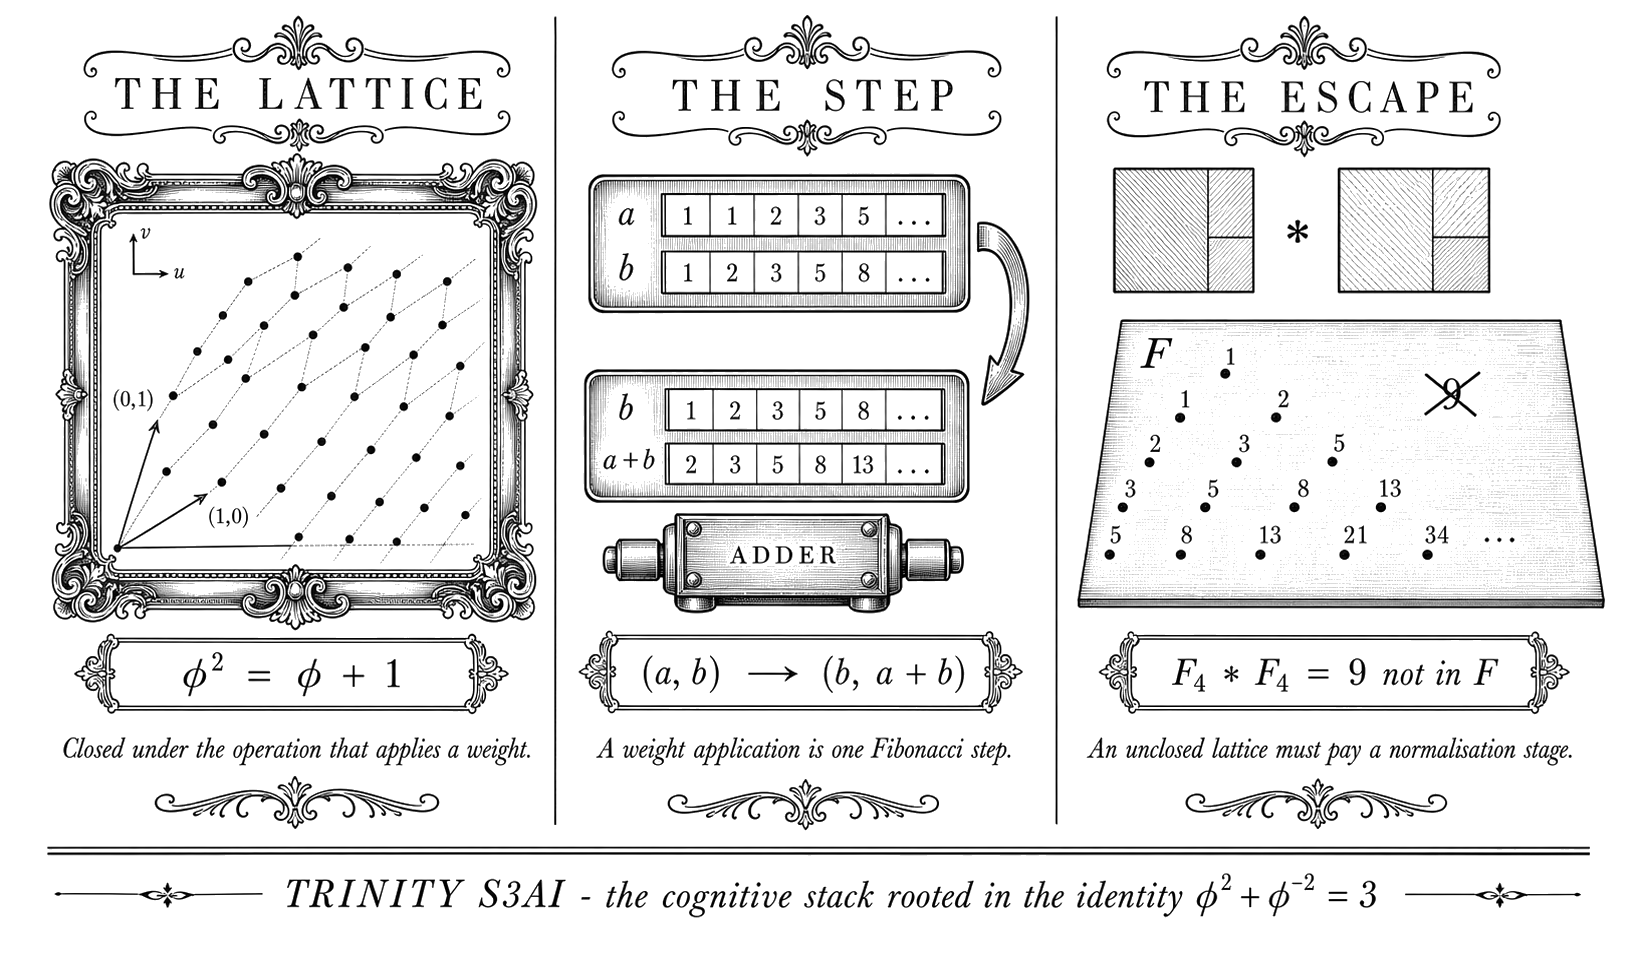
\includegraphics[width=\textwidth]{canon/canon-tnf-04-closure.png}
\caption{Why the alphabet is $\varphi$. The lattice $\mathbb{Z}[\varphi]$ is closed because $\varphi^2=\varphi+1$; the step is a Fibonacci shift $(a,b)\mapsto(b,a+b)$; and the escape is immediate elsewhere, since $F_4\cdot F_4=9\notin F$.}
\label{fig:canon-closure}
\end{figure}

\subsection{How many multiply-free scales are there}\label{sec:hierarchy}

Closure explains why $\varphi$ works. It does not by itself say $\varphi$ is the
only choice, and the honest answer is that it is not --- it is the only choice at
its size.

A scale $r$ can be applied without a multiplier exactly when $r$ is an algebraic
integer whose companion matrix has entries in $\{0,\pm1\}$: writing
$r^{d}=a_{d-1}r^{d-1}+\dots+a_0$, multiplication by $r$ maps the coordinate
vector $(x_0,\dots,x_{d-1})$ to $(a_0x_{d-1},\;x_0+a_1x_{d-1},\;\dots)$, and any
$|a_i|>1$ reintroduces a constant multiply. The condition is finite, so the
scales can be enumerated rather than argued about.

\begin{theorem}[The multiply-free scales, by degree]\label{thm:hierarchy}
Over coefficients in $\{0,\pm1\}$:
\begin{itemize}
\item \textbf{Degree 1} admits $r\in\{0,\pm1\}$, which is no scaling, and
      $r=\pm2^k$, free by shifting. One register, ratio $2$.
\item \textbf{Degree 2} admits exactly two equations with a real root of modulus
      other than $0$ or $1$: $r^2=r+1$ and $r^2=-r+1$, whose roots are $\varphi$
      and $\varphi^{-1}$ --- the same ladder. One addition, two registers,
      ratio $1.618$.
\item \textbf{Degree 3} admits three: $r^3=r+1$ (plastic, $1.3247$),
      $r^3=r^2+1$ (supergolden, $1.4656$), $r^3=r^2+r+1$ (tribonacci,
      $1.8393$). At most two additions, three registers.
\end{itemize}
\end{theorem}
\begin{proof}
Exhaustive over the nine degree-2 and twenty-seven degree-3 coefficient triples;
the degree-2 discriminants $a^2+4b$ are negative for four cases, and the
remaining five give roots in $\{0,\pm1\}$ except for $b=1,a=\pm1$.
\end{proof}

\begin{corollary}\label{cor:nothing-between}
Nothing lies between the shift and $\varphi$. $\varphi$ is the unique
multiply-free refinement of the power-of-two ladder available at two registers.
\end{corollary}
\begin{proof}
At degree two the companion polynomial has the form
$r^2-ar-b=0$ with $a,b\in\{-1,0,1\}$, so there are nine coefficient pairs.
The discriminant is $a^2+4b$.  Direct enumeration leaves only
$(a,b)=(1,1)$ and $(-1,1)$ with a real root whose modulus exceeds one;
their roots are respectively $\varphi$ and $-\varphi$.  The other real
roots have modulus at most one, or give the trivial zero or unit scales.
Thus the positive two-register refinement is $\varphi$, while the preceding
shift ladder has ratio $2$ by the degree-one case of
Theorem~\ref{thm:hierarchy}.
\end{proof}

So the multiply-free scale is not a point but a hierarchy indexed by algebraic
degree, and each degree buys finer granularity for one more register.
Table~\ref{tab:hierarchy} measures the trade at the first two rungs where it is
a trade at all. The plastic step
$(a,b,c)\mapsto(c,\,a+c,\,b)$ costs the same single addition as the Fibonacci
step and one more register, and its ladder is finer: successive levels differ by
$13.97\%$ against $\varphi$'s $23.61\%$.

\begin{table}[t]\centering
\caption{One scale application, xc7a200t, median of five seeds. Matched: neither
unit has a direction mux. Level error is $(r-1)/(r+1)$, the worst relative gap
on a ladder of ratio $r$, and is analytic in $r$ rather than measured. $^{\ast}$:
this frequency is stated in no record file in the repository at this revision,
where the other three rows are ---
\texttt{ONE\_\allowbreak ADDER\_\allowbreak FAMILY\_\allowbreak 2026-08-10.md} and
\texttt{LADDER\_\allowbreak COST\_\allowbreak AND\_\allowbreak LAW\_\allowbreak 2026-08-10.md} --- so it is illustrative and carries
no hardware-performance claim. The 32-bit comparison in the text uses the two rows
that do have records.}
\label{tab:hierarchy}
\begin{tabular}{lrrrr}
\toprule
scale & LUT & FF & $F_{\max}$ (MHz) & level error \\
\midrule
$\varphi$, 16-bit          & \textbf{149} & 128 & 307.69 & $23.61\%$ \\
plastic, 16-bit            & 186 & 160 & $318.47^{\ast}$ & $\mathbf{13.97\%}$ \\
\addlinespace
$\varphi$, 32-bit          & \textbf{223} & 192 & \textbf{247.10} & $23.61\%$ \\
plastic, 32-bit            & 228 & 200 & 231.21 & $\mathbf{13.97\%}$ \\
\bottomrule
\end{tabular}
\end{table}

At 32 bits the refinement costs $2.2\%$ of the area and $6.4\%$ of the
frequency. That is close enough to free that the choice is a question about the
network rather than about the arithmetic, so we asked the network.


\begin{figure}[htbp]\centering
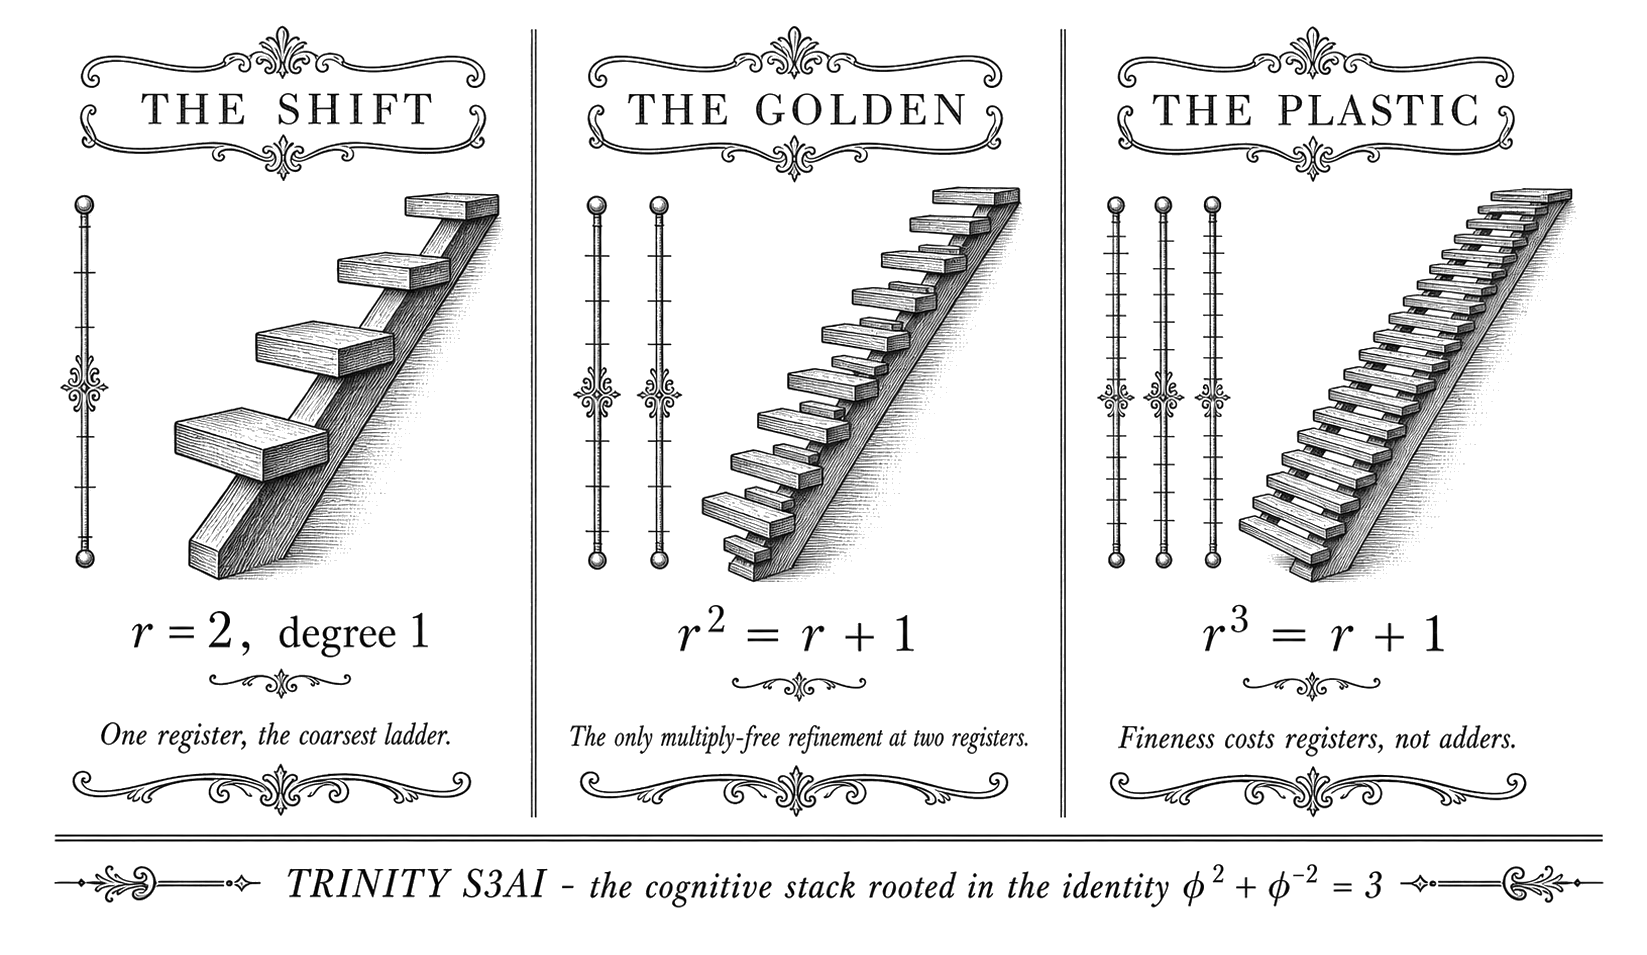
\includegraphics[width=\textwidth]{canon/canon-tnf-05-hierarchy.png}
\caption{How many multiply-free scales there are. The shift, the golden step, and the plastic step are rungs of one family $r^d=r+1$; degree two admits $\varphi$ alone.}
\label{fig:canon-hierarchy}
\end{figure}


% ---- tnf_paper.tex lines 4360-4815: Fineness costs registers, not adders ----
\section{Fineness costs registers, not adders}\label{sec:oneadder}

\triptych{canon-tnf-28-oneadder.png}{Fineness costs registers, not adders.}{fig:canon-oneadder}


Reading the hierarchy by degree, and taking the cost to be the minimal ratio
available at each degree, hides the result. Read along a family instead.

\paragraph{What is forced, and what is not.} For base $\varphi$, three digits is
the proven minimum for constant-time carry-free addition~\cite{frougny2011,
frougny2013}; a two-digit alphabet is impossible. $\{-1,0,1\}$ is \emph{one} of
the minimal alphabets --- chosen because it is symmetric, so subtraction reuses
the adder --- and not the unique one: $\{0,1,2\}$ is minimal too, and a working
$\{0,1,2\}$ parallel adder for $\varphi$ was implemented and tested here.
L\'egersk\'y~\cite{legersky2018} extends the bound to any finite alphabet inside
$\mathbb{Z}[\varphi]$ containing zero, so no non-integer set escapes it.

The bound constrains the \emph{digit} alphabet of a positional representation
and one operation --- rewriting a digit-wise sum back into the alphabet with a
sliding window. A weight set has no base and no carry, so it does not transfer
to the weight alphabet of a dot product. It would transfer only if the
accumulator were itself a redundant base-$\varphi$ positional format, and ours
is a pair of integers never reduced to a digit string. We record the theorem
because it says something real and narrow --- two letters cannot be made to work
at any window size --- and record its scope because the wider reading, which we
first wrote down, is false.

The window is not small either: the published algorithm on $\{-1,0,1\}$ is
$21$-local, with memory $10$ and anticipation $10$. ``Constant time'' read as
``cheap'' would be wrong by an order of magnitude.

\begin{table}[t]\centering
\caption{The multiply-free scales in one place. Level error is $(r-1)/(r+1)$,
the worst relative gap on a ladder of ratio $r$; LUT area is one scale
application at 16-bit components, xc7a200t, median of five seeds. Every rung
below the shift costs exactly one addition; only the register count grows.}
\label{tab:allscales}
\begin{tabular}{llrrrrl}
\toprule
scale & polynomial & $r$ & regs & adds & level err. & LUT / $F_{\max}$ \\
\midrule
shift        & $r=2$              & $2.0000$ & 1 & 0 & $33.33\%$ & --- \\
$\varphi$    & $r^2=r+1$          & $1.6180$ & 2 & 1 & $23.61\%$ & $149$ / $307.69$ \\
supergolden  & $r^3=r^2+1$        & $1.4656$ & 3 & 1 & $18.88\%$ & --- \\
plastic      & $r^3=r+1$          & $1.3247$ & 3 & 1 & $13.97\%$ & $228$ / $231.21$ \\
             & $r^5=r^3+1$        & $1.2365$ & 5 & 1 & $10.57\%$ & $164$ / $306.56$ \\
             & $r^4{=}{-}r^3{+}r^2{+}r{+}1$ & $1.1787$ & 4 & 3 & $8.20\%$ & $469$ / $184.98$ \\
             & $r^6=r+1$          & $1.1347$ & 6 & 1 & $6.31\%$ & --- \\
             & $r^8=r+1$          & $1.0970$ & 8 & 1 & $4.63\%$ & $225$ / $815.66$ \\
\bottomrule
\end{tabular}
\end{table}

\paragraph{A qualification the table needs.} Not every rung is Perron --- that
is, not every one has its real root strictly dominant among the conjugates. The
degree-4 minimum has a conjugate of modulus $1.5129$ against a root of
$1.1787$, and the degree-6 minimum $1.3069$ against $1.0863$; the degree-5
minimum $1.1237$ is Perron, its largest conjugate being $1.0959$. Where the
root is not dominant, the coordinate vector of $r^{k}$ grows as the larger
conjugate rather than as the value, so a chain of $k$ applications needs
$k\log_2(\rho/r)$ guard bits --- $0.36$ bits per step at degree 4. That is a cost
on composition and not on a single application, which is why the LUT-area column
does not show it, and it is stated here rather than left for a reader to find.

Wu's exhaustive search~\cite{wu2010} establishes that $1.123732821$ is the
smallest Perron number of degree 5, so the degree-5 rung is provably optimal
among Perron scales. It is also the Lind--Boyd exceptional case: the family
$r^d=r+1$ is Lind's conjectured smallest Perron number of degree $d$, corrected
by Boyd~\cite{boyd1985} at exactly $d>3$ with $d\equiv3,5 \pmod 6$. The
exceptional minimisers are finer --- $1.1237$ against the family's $1.1673$ at
$d=5$ --- but they are not one-adder: they cost $3$, $5$, $7$ and more adders as
$d$ grows, and beyond $d=5$ the gain is under $0.8\%$. A finer rung at five
adders is a different trade from a finer rung at one, and only the second would
have been news.

Table~\ref{tab:allscales} collects them. Two readings are worth making
explicit. Along the one-adder family the adder count is constant and only the
registers grow, so the row for $r^4$ --- three adders for a finer ratio than
$r^5$ gives with one --- is the exception rather than the pattern, and it is what
made an earlier reading of this hierarchy report a cost that grows with degree.
And the frequency column does not fall as the ratio does: the $d=8$ rung
measures $815.66$\,MHz against $\varphi$'s $307.69$, because its single adder
sits on one of eight parallel paths rather than one of two.

\begin{theorem}[Siegel's floor bounds the family]\label{thm:siegel}
A Pisot--Vijayaraghavan number is a real algebraic integer above one whose
conjugates all lie strictly inside the unit circle. Siegel~\cite{siegel1944}
proved the smallest is $1.3247179572\ldots$, the root of $r^3=r+1$, at any
degree and with any integer coefficients. That root is the degree-3 member of
the family below, so the family is Pisot at $d=2$ and $d=3$ and at no higher
degree: every later member is finer than Siegel's floor and therefore cannot be
Pisot.
\end{theorem}
\begin{proof}
For $d=2$, the positive root is $\varphi=1.618033\ldots$ and the other root is
$-\varphi^{-1}$, so its conjugate has modulus below one. For $d=3$, the
positive root is $\rho=1.324717957\ldots$; the product of the two remaining
conjugates is $\rho^{-1}$, so their common modulus is
$1/\sqrt{\rho}=0.868837\ldots<1$. For $d\ge4$, since
$\rho^d>\rho^3=\rho+1$, the root of $x^d-x-1$ lies strictly below $\rho$.
Siegel's lower bound says that no Pisot number lies below $\rho$, so no such
later root is Pisot. This proves the asserted boundary, using Siegel's theorem
for the external lower-bound step.
\end{proof}

Computed conjugate moduli agree exactly: $0.6180$ at $d=2$, $0.8688$ at $d=3$,
then $1.0633$, $1.0990$, $1.0992$, $1.0920$, $1.0837$ at $d=4\ldots8$. The
boundary is not an accident of our enumeration; it is where a theorem from 1944
says it must be, and \emph{the finest scale that is both applicable by one
addition and Pisot is the plastic number.}

The distinction matters for what may be built on a rung, not for the arithmetic
itself. Normalisation in base $\theta$ is realisable by a finite automaton
exactly when $\theta$ is Pisot~\cite{berend1994}, and for $n\ge4$ the root of
$x^n = x+1$ is not even a Parry number, its shift being
non-sofic~\cite{akiyama2016}. So a bounded-latency renormaliser or a
canonical-form comparator exists at $d=2$ and $d=3$ and provably not above.
Nothing in this paper's datapath normalises --- the coordinates are carried as
integers and never reduced to a canonical digit string --- which is why the
$d=8$ step measures $815.66$\,MHz rather than failing to close. We state it
because a reader who assumes a normaliser would be assuming something the
mathematics forbids.

\begin{theorem}[The one-adder family]\label{thm:oneadder}
For every integer $d\geq2$ the polynomial $r^{d}=r+1$ has a unique real root above one. It
has exactly two non-zero coefficients, so its companion map is
\[
  (x_0,\dots,x_{d-1}) \;\mapsto\; (x_{d-1},\; x_0+x_{d-1},\; x_1,\dots,x_{d-2}),
\]
\emph{one addition} regardless of $d$, and the roots converge to $2^{1/d}$ from
above. Any granularity a logarithmic subdivision offers is therefore reachable
without a multiplier, at the cost of registers alone.
\end{theorem}
\begin{proof}
For $d\geq2$, $f(r)=r^d-r-1$ is negative at $r=1$ and positive at $r=2$,
so a root lies in $(1,2)$. Since $f'(r)=dr^{d-1}-1>0$ for $r\geq1$,
that root is unique. The displayed companion matrix has only the two
non-zero polynomial coefficients, hence its only arithmetic operation is the
sum $x_0+x_{d-1}$; the other entries are wires and registers. The root is
strictly above $2^{1/d}$ because $r^d=r+1>2$. Finally, for any
$\varepsilon>0$, $(1+\varepsilon)^d>2+\varepsilon$ for all sufficiently
large $d$, so the root is below $1+\varepsilon$; hence it tends to $1$,
as does $2^{1/d}$, and the difference tends to zero.
\end{proof}

The map is verified exact over $3000$ random coordinate vectors at $d=5$ and
$d=8$. The convergence is quick: $r/2^{1/d}$ is $1.1441$ at $d=2$, $1.0159$ at
$d=5$, $1.0059$ at $d=8$ and $1.0014$ at $d=16$.

\paragraph{The ladder's cost depends on its role.} Applying a ladder weight
$r^{-j}$ costs $j$ steps of the companion map. As a \emph{block scale} that is
one value per thirty-two weights and the steps amortise; as an \emph{element} it
is paid per weight, and a six-bit ladder needs $j$ up to $31$. The element form
is therefore a coordinate table --- the code selects a vector in
$\mathbb{Z}[r]$ directly --- and Table~\ref{tab:elemsil} prices it against what
it buys.

\paragraph{The assembled node.} Every fabric-area figure above prices a part. The
figure asked from outside is LUTs per neuron, and Table~\ref{tab:node} is the
assembled thing: fan-in $N$, weights from the alphabet, accumulator in
$\mathbb{Z}[\varphi]$, 8-bit samples, harness subtracted.

\begin{table}[t]\centering
\caption{A complete ternary neuron, xc7a200t, median of five seeds, harness
subtracted, \texttt{-nodsp}. The first column is the implementation this paper
first built; the second folds the negation into the accumulation tree, which is
where it belonged.}
\label{tab:node}
\begin{tabular}{lrrrrr}
\toprule
fan-in & LUT/weight & folded & $F_{\max}$ & folded & DSP \\
\midrule
8  & $82.5$ & $\mathbf{28.0}$ & $109.35$ & $87.29$ & \textbf{0} \\
16 & $87.1$ & $\mathbf{33.1}$ & $91.43$ & $73.42$ & \textbf{0} \\
32 & $119.0$ & $\mathbf{33.2}$ & $66.53$ & $58.22$ & \textbf{0} \\
\bottomrule
\end{tabular}
\end{table}

Two's complement is $(\lnot x)+1$ and the $+1$ of every lane is a single bit, so
the fold is an exclusive-or with the weight's sign plus a narrow second tree
carrying the ones, added once at the root. Equivalence was checked before
synthesis: $0$ mismatches in $400$ random $(x,w)$ vectors. Area falls by
$2.9$--$3.6\times$ and lands on the hand count --- a three-way select of a
16-bit value at roughly $16$ LUT6 plus a 16-bit add at roughly $8$, so $24$ to
$30$ per lane --- which is what confirms the negation was the whole gap rather
than part of it. Frequency falls about $20\%$, the carry tree's root addition
sitting after the main one; on throughput per area the trade is worth
$2.35$--$2.87\times$.

So a ternary neuron costs \textbf{28 LUT per weight at fan-in 8 and no DSP at
any fan-in}.

\paragraph{And one pipeline register, where it pays.} The critical path is the
whole adder tree, so cutting it once at the halfway level trades a cycle and
$N/2$ registers for frequency --- worth measuring rather than assuming, and the
answer is not uniform. Equivalence checked first: $0$ mismatches in $398$ random
$(x,w)$ vectors, the pipelined output trailing by exactly one cycle.

\begin{table}[t]\centering
\caption{One pipeline cut in the accumulation tree. The register cost overtakes
the frequency gain between sixteen and thirty-two, so the unpipelined form is
the better one at fan-in 32 --- the opposite of the usual advice, which is why it
was measured.}
\label{tab:nodepipe}
\begin{tabular}{lrrr}
\toprule
fan-in & LUT/weight & $F_{\max}$ (MHz) & MHz per LUT \\
\midrule
8  & $28.0\to\mathbf{32.4}$ & $87.29\to\mathbf{126.73}$ & $0.390\to0.489$ (\textbf{$+25.6\%$}) \\
16 & $33.1\to\mathbf{34.9}$ & $73.42\to\mathbf{106.38}$ & $0.139\to0.191$ (\textbf{$+37.6\%$}) \\
32 & $33.2\to47.3$ & $58.22\to75.68$ & $0.055\to0.050$ ($-8.7\%$) \\
\bottomrule
\end{tabular}
\end{table}

At fan-in 8 and 16 the cut buys $45\%$ more frequency for $16\%$ and $5\%$ more
area; at 32 it buys $30\%$ for $42\%$. The crossover is where $N/2$ registers
stop being cheap relative to the tree they cut. The configuration to quote is
therefore fan-in 8 or 16 with one stage: $32.4$ LUT per weight at $126.73$\,MHz,
or $34.9$ at $106.38$, both at zero DSP. We report the unfolded column beside it because that number was
published first, with a caveat naming the negation as its likely cause, and the
cause turned out to be the whole of it.

\begin{table}[t]\centering
\caption{Element decoders as coordinate tables, isolated, median of five seeds,
against the perplexity of the same ladder on SmolLM2-135M
(\texttt{fp32} baseline $14.3607$). Thirty-three more LUTs move the error from
$70\%$ to $3.7\%$ at no cost in frequency.}
\label{tab:elemsil}
\begin{tabular}{lrrrrr}
\toprule
decoder & table & LUT & $F_{\max}$ & ppl & above \texttt{fp32} \\
\midrule
$\varphi$, 4-bit          & $7\times2\times5$b  & \textbf{89} & $621.89$ & $24.4280$ & $+70.1\%$ \\
$r^5{=}r^3{+}1$, 5-bit    & $15\times5\times4$b & $95$ & $482.39$ & $15.9242$ & $+10.9\%$ \\
$r^6{=}r{+}1$, 6-bit      & $31\times6\times5$b & $122$ & $612.00$ & $\mathbf{14.8882}$ & $\mathbf{+3.7\%}$ \\
\bottomrule
\end{tabular}
\end{table}

The middle rung is the one a budget would choose: five bits and $95$ LUT for
$+10.9\%$, a six-LUT premium over $\varphi$ for a sixfold reduction in error.
Applying the scale remains one addition throughout and the datapath remains free
of DSP.

\begin{table}[t]\centering
\caption{One scale application, 16-bit components, xc7a200t, median of five
seeds. A fivefold refinement costs $51\%$ more LUTs and no frequency: the
eight-register step's single adder sits on one of eight parallel paths rather
than one of two.}
\label{tab:oneadder}
\begin{tabular}{lrrrrr}
\toprule
step & LUT & FF & $F_{\max}$ & level error & adds \\
\midrule
$\varphi$, $r^2=r+1$   & \textbf{149} & 128 & $307.69$ & $23.607\%$ & 1 \\
$r^5=r^3+1$            & $164$ & 160 & $306.56$ & $10.575\%$ & 1 \\
$r^8=r+1$              & $225$ & 212 & $\mathbf{815.66}$ & $\mathbf{4.625\%}$ & 1 \\
\bottomrule
\end{tabular}
\end{table}

Measured as a block scale on two networks, the one-adder ratio matches the
geometric ratio beside it at both widths: at five bits $21.5040$ against
$21.5872$ on SmolLM2 and $14.7342$ against $14.7814$ on Qwen, at six bits
$19.3209$ against $20.0199$ and $13.8528$ against $13.8915$. The geometric
grid's advantage of \record{the geometric-scale theorem} is therefore available with no
multiplier at all.

This also resolves the tension left by \record{the geometric-scale theorem}. The grid
minimising relative error is geometric with ratio $R^{1/N}$, an arbitrary real
needing a multiplier --- in general. Where a block scale actually lives, the
occupied range being $8.32$ to $9.12$ binades and the width four to six bits,
the nearest multiply-free ratio matches the optimum to within $0.06\%$:
$1.551532$ against $1.551145$ at four bits, $1.236506$ against $1.236662$ at
five, $1.110187$ against $1.110180$ at six. At eight bits our first enumeration reported a gap, and that was our own search
bound rather than a property of the spectrum: stopping at degree $8$ the nearest
ratio was $1.049852$ against a target of $1.026159$, while degree $9$ reaches
$1.036380$ and degree $10$ reaches $1.027738$. Allowing coefficients in
$\{0,\pm1,\pm2\}$ --- still addition and wiring, since $\pm2$ is a shift ---
degree $9$ reaches $1.026129$, within $0.003\%$, out of $734{,}533$ enumerated
roots.

What is a real limit is the one-adder family itself. At the same eight-bit
target its best member is $1.0850702$ under $\{0,\pm1\}$ and $1.0510545$ under
$\{0,\pm1,\pm2\}$, errors of $5.6\%$ and $2.4\%$, and these do not improve with
degree. Any ratio is reachable multiply-free if adders are spent; a coarser set
is reachable with one.

\paragraph{The hierarchy is cheap only as far as degree three.}
Table~\ref{tab:deg4} adds the smallest degree-4 scale, the root of
$r^4=-r^3+r^2+r+1$, whose map $(x_0,x_1,x_2,x_3)\mapsto(x_3,\,x_0{+}x_3,\,
x_1{+}x_3,\,x_2{-}x_3)$ was verified exact over $3000$ random coordinate
vectors.

\begin{table}[t]\centering
\caption{One scale application, xc7a200t, 32-bit, median of five seeds. Degrees
2 and 3 both cost one addition; at degree 4 the coefficient vector stops being
sparse and the cost jumps.}
\label{tab:deg4}
\begin{tabular}{lrrrrr}
\toprule
scale & LUT & FF & $F_{\max}$ & level error & add/sub \\
\midrule
$\varphi$ (deg 2)      & \textbf{223} & 192 & \textbf{247.10} & $23.61\%$ & 1 \\
plastic (deg 3)        & 228 & 200 & 231.21 & $13.97\%$ & 1 \\
$1.1787$ (deg 4)       & 469 & 320 & 184.98 & $\mathbf{8.20\%}$ & 3 \\
\bottomrule
\end{tabular}
\end{table}

This places the alphabet exactly. $\varphi$ is the right rung at four bits,
where $r^{*}=1.4115$ falls between it and supergolden and the two tie. It is the
wrong rung at five and above --- and by five, the affordable part of the
hierarchy has been left behind too, since degree 4 costs $2.1\times$ the area.
The regime in which a multiply-free datapath is worth building is the one where
degrees 2 and 3 are the only rungs one can pay for, and that regime is three to
five bits.

A first predictor failed and the failure is informative: choosing the finest
ladder whose span covers the weights' channel dynamic range --- $268.95\times$
median over $155{,}520$ channels --- selects the coarsest rung at every budget,
correct at three bits and wrong at four and five. Coverage is the wrong
criterion because clipping the smallest weights is nearly free while rounding
the largest is not. The quantity that decides is total error, and total error is
computable before any model runs.

The distinction is between quantizing to \emph{Fibonacci numbers} and working in
\emph{the ring those numbers are the coordinates of}. It is narrower than it may
sound, and we state it narrowly: by Binet's formula $F_n = \operatorname{round}
(\varphi^{n}/\sqrt5)$ exactly for $n \ge 1$ --- verified here to $n = 25$ --- so a
Fibonacci ladder \emph{is} a $\varphi$-power ladder up to a constant offset. What
does not follow is closure. $F_iF_j$ is not a Fibonacci number, so the product
leaves the representable set; $\varphi\,(a+b\varphi)$ stays in
$\mathbb{Z}[\varphi]$. The two schemes agree on the ladder and differ on the
ring, and the transformation stage is the price of the second. $F_iF_j$ escapes the set;
$\varphi\cdot(a+b\varphi)$ does not. What the escape costs is exactly the two
adders and the routing scheme, and what closure buys is that neither is needed:
one integer addition, and the multiply-free path is not an approximation of a
multiply but equal to it (Theorem~\ref{thm:exact}).

The closure half of this argument is machine-checked. In the accompanying
development the map $(a,b)\mapsto(b,a+b)$ is proved to compute multiplication by
$\varphi$ on the reals, and the exactness of an entire dot product follows from
it, in Coq with no admitted lemmas.

\paragraph{The stage costs an order of magnitude, and it runs per accumulation.}
Corollary~\ref{cor:closure} says a stage is required; the fabric says what it
costs. Table~\ref{tab:closure} measures one accumulation step in the harness of
Section~\ref{sec:hardware} --- isolated unit, every output bit folded into the
observed reduction, median of five placement seeds.

\begin{table}[t]\centering
\caption{One accumulation step, xc7a200t, median of five seeds. The non-closed
unit is the greedy Zeckendorf normaliser, oracle-checked exhaustively over all
$65{,}536$ inputs for the sum, the no-two-adjacent-digits property, and
agreement with an independently written greedy model.}
\label{tab:closure}
\begin{tabular}{lrr}
\toprule
one accumulation & LUT & $F_{\max}$ (MHz) \\
\midrule
closed, $\mathbb{Z}[\varphi]$, componentwise (16-bit) & \textbf{182} & \textbf{299.94} \\
non-closed, normalise back (16-bit)                   & 1756 & 11.46 \\
\addlinespace
closed, $\mathbb{Z}[\varphi]$, componentwise (32-bit) & \textbf{283} & \textbf{239.35} \\
non-closed, normalise back (32-bit)                   & 7017 & 4.25 \\
\bottomrule
\end{tabular}
\end{table}

The stage does not run once per multiply. A product can be handled either way:
the identity $F_mF_n = \bigl(L_{m+n}-(-1)^nL_{m-n}\bigr)/5$ turns one into two
table lookups and a subtraction. It is \emph{accumulation} that has no such
escape, because the sum of two representable numbers is not representable ---
$F_3+F_3 = 4 = F_4+F_1$, and the representation changes non-trivially. At fan-in
$512$ the stage runs $512$ times per neuron, against a pair of integer registers
on the closed side.

One limit is worth stating: greedy normalisation is not proved to be the
cheapest --- constant-time Zeckendorf adders exist --- so the ratio is an upper
bound on this implementation, while Corollary~\ref{cor:closure} carries the
qualitative claim.

The other apparent limit does not survive measurement. Part of the frequency gap
is combinational depth, $46$ dependent stages against one addition, and
pipelining should convert that into latency and registers. It does, and it is
not enough: swept to $32$ stages at 16 bits and $48$ at 32, frequency rises and
then plateaus at $249.44$ and $111.36$\,MHz against the closed path's $299.94$
and $239.35$, the second less than half. There is a reason.

\begin{theorem}[The normalisation floor]\label{thm:normfloor}
A normalisation cascade cannot be pipelined below one compare-and-subtract per
stage, so its clock period is bounded below by the carry latency of a
compare-and-subtract at the datapath width. A compare-and-subtract is strictly
more than an addition --- a subtraction plus the comparison selecting it --- so
the floor of a non-closed path lies above the floor of a closed path whose step
is a single addition.
\end{theorem}
\begin{proof}
In the stated cascade, a stage must first compare the current residue with its
threshold and then subtract that threshold when the comparison selects it.
The select bit is data-dependent, so the subtraction cannot be completed before
the comparison; these two operations form one serial dependency at the
datapath width. Inserting a register between them does not shorten the
compare-and-subtract step: it creates an additional pipeline stage and carries
the decision as state. The closed path has one data-dependent operation per
step, namely the addition. Thus, under the same datapath and register model,
the non-closed stage has a strictly longer carry dependency than the closed
stage; this is a lower bound on the period, not a claim about a particular
place-and-route result.
\end{proof}

At the plateau the trade is $7.8\times$ and $19.7\times$ the area,
$3.6\times$ and $8.3\times$ the registers, $32$ and $48$ cycles of latency, and
still the lower frequency.


This is a different kind of statement from the rest of the paper. Everywhere else
we compare error magnitudes between formats; here there is no error to compare.
Rounding enters a $\varphi$-ternary network only at the nonlinearity, where it is
unavoidable in any format, and the cost of exactness in the linear path is two
integer accumulators in place of one floating-point one.

\paragraph{Why the alphabet base cannot be anything else.} Closure requires
$r^{2} = pr + q$ with $p,q$ integers, so that $\mathbb{Z}[r]$ is a ring. Among
such $r>1$ the cheapest recurrence is the one with $p=q=1$, since any larger $p$
introduces a shift alongside the addition: $r = 1+\sqrt2$ satisfies
$r^2 = 2r+1$ and costs a shift, while $r=\sqrt2$ has $r^2 = 2$ and loses the
scale out of the lattice entirely. The $p=q=1$ case is $\varphi$, and it is the
minimum rather than a member of a set of acceptable choices.

\paragraph{Scope, stated so the claim does not overreach.} This concerns
arithmetic in a lattice. It applies to the linear algebra that dominates a
network's work and its LUT-area cost, and it says nothing about control flow,
addressing or branching, which are not lattice problems and gain nothing from
\triptych{canon-tnf-57-conjugatetoll.png}{Along the scale hierarchy, conjugate growth can add guard bits under composition, and exceptional finer roots exchange their gain for several adders.}{fig:canon-b4-57conjugatetoll}

$\varphi$.
\triptych{canon-tnf-56-carryalphabet.png}{The carry-free digit result requires a three-symbol positional alphabet and a 21-local rewriting window, while the weight alphabet is outside that scope.}{fig:canon-b4-56carryalphabet}



